%%%%%% Run at command line, run
%%%%%% xelatex grad-sample.tex 
%%%%%% for a few times to generate the output pdf file
\documentclass[12pt,oneside,openright,a4paper]{cpe-english-project}

\usepackage{polyglossia}
\setdefaultlanguage{english}
\setotherlanguage{thai}
\newfontfamily\thaifont[Script=Thai,Scale=1.23]{TH Sarabun New}

%%%%%% add package for gantt chart
\usepackage{xcolor,colortbl}
\usepackage{forloop}
\newcounter{loopcntr}
\newcommand{\rpt}[2][1]{%
  \forloop{loopcntr}{0}{\value{loopcntr}<#1}{#2}%
}
\newcommand{\on}[1][1]{
  \forloop{loopcntr}{0}{\value{loopcntr}<#1}{&\cellcolor{gray}}
}
\newcommand{\off}[1][1]{
  \forloop{loopcntr}{0}{\value{loopcntr}<#1}{&}
}

%%%%% add package multirole for table
\usepackage{multirow}

\defaultfontfeatures{Mapping=tex-text,Scale=1.0,LetterSpace=0.0}
\setmainfont[Scale=1.0,LetterSpace=0,WordSpace=1.0,FakeStretch=1.0]{Times New Roman}
\setmathfont(Digits)[Scale=1.0,LetterSpace=0,FakeStretch=1.0]{Times New Roman}


%%%%%%%%%%%%%%%%%%%%%%%%%%%%%%%%%%%%%%%%%%%%%%%%%%%%%%%%%%%%%%%%%%%
% Customize below to suit your needs 
% The ones that are optional can be left blank. 
%%%%%%%%%%%%%%%%%%%%%%%%%%%%%%%%%%%%%%%%%%%%%%%%%%%%%%%%%%%%%%%%%%%
% First line of title
\def\disstitleone{Project No. 50}   
% Second line of title
\def\disstitletwo{NKR: On top scheduler for Apache Mesos}   
% Your first name and lastname
\def\dissauthor{Ms.Pasinee Santivorranant}   % 1st member
%%% Put other group member names here ..
\def\dissauthortwo{Mr.Supapat Sri-on}   % 2nd member (optional)
\def\dissauthorthree{Ms.Parattha Weerapong}   % 3rd member (optional)


% The degree that you're persuing..
\def\dissdegree{Bachelor of Engineering} % Name of the degree
\def\dissdegreeabrev{B.Eng} % Abbreviation of the degree
\def\dissyear{2020}                   % Year of submission
\def\thaidissyear{2563}               % Year of submission (B.E.)

%%%%%%%%%%%%%%%%%%%%%%%%%%%%%%%%%%%%%%%%%%%%
% Your project and independent study committee..
%%%%%%%%%%%%%%%%%%%%%%%%%%%%%%%%%%%%%%%%%%%%
\def\dissadvisor{Asst Prof.Rajchawit Sarochawikasit}  % Advisor
%%% Leave it empty if you have no Co-advisor
\def\disscoadvisor{}  % Co-advisor
\def\disscommitteetwo{Asst Prof. Dr. Khajonpong Akkarajitsakul}  % 3rd committee member (optional)
\def\disscommitteethree{Asst Prof. Dr. Phond Phunchongharn}   % 4th committee member (optional) 
\def\disscommitteefour{Asst Prof. Sanan Srakaew}    % 5th committee member (optional) 

\def\worktype{Project} %%  Project or Independent study
\def\disscredit{3}   %% 3 credits or 6 credits


\def\fieldofstudy{Computer Engineering} 
\def\department{Computer Engineering} 
\def\faculty{Engineering}

\def\thaifieldofstudy{วิศวกรรมคอมพิวเตอร์} 
\def\thaidepartment{วิศวกรรมคอมพิวเตอร์} 
\def\thaifaculty{วิศวกรรมศาสตร์}
 
\def\appendixnames{Appendix} %%% Appendices or Appendix

\def\thaiworktype{ปริญญานิพนธ์} %  Project or research project % 
\def\thaidisstitleone{หัวข้อปริญญานิพนธ์บรรทัดแรก}
\def\thaidisstitletwo{หัวข้อปริญญานิพนธ์บรรทัดสอง}
\def\thaidissauthor{นางสาวภาสินี สันติวรนันท์}
\def\thaidissauthortwo{นายศุภพัฒน์ ศรีอ่อน} %Optional
\def\thaidissauthorthree{นางสาวปรัษฐา วีระพงษ์} %Optional

\def\thaidissadvisor{ผศ.ราชวิชช์ สโรชวิกสิต}
%% Leave this empty if you have no co-advisor
\def\thaidisscoadvisor{} %Optional
\def\thaidissdegree{วิศวกรรมศาสตรบัณฑิต}

% Change the line spacing here...
\linespread{1.15}

%%%%%%%%%%%%%%%%%%%%%%%%%%%%%%%%%%%%%%%%%%%%%%%%%%%%%%%%%%%%%%%%
% End of personal customization.  Do not modify from this part 
% to \begin{document} unless you know what you are doing...
%%%%%%%%%%%%%%%%%%%%%%%%%%%%%%%%%%%%%%%%%%%%%%%%%%%%%%%%%%%%%%%%


%%%%%%%%%%%% Dissertation style %%%%%%%%%%%
%\linespread{1.6} % Double-spaced  
%%\oddsidemargin    0.5in
%%\evensidemargin   0.5in
%%%%%%%%%%%%%%%%%%%%%%%%%%%%%%%%%%%%%%%%%%%
%\renewcommand{\subfigtopskip}{10pt}
%\renewcommand{\subfigbottomskip}{-5pt} 
%\renewcommand{\subfigcapskip}{-6pt} %vertical space between caption
%                                    %and figure.
%\renewcommand{\subfigcapmargin}{0pt}

\renewcommand{\topfraction}{0.85}
\renewcommand{\textfraction}{0.1}

\newtheorem{theorem}{Theorem}
\newtheorem{lemma}{Lemma}
\newtheorem{corollary}{Corollary}

\def\QED{\mbox{\rule[0pt]{1.5ex}{1.5ex}}}
\def\proof{\noindent\hspace{2em}{\itshape Proof: }}
\def\endproof{\hspace*{\fill}~\QED\par\endtrivlist\unskip}
%\newenvironment{proof}{{\sc Proof:}}{~\hfill \blacksquare}
%% The hyperref package redefines the \appendix. This one 
%% is from the dissertation.cls
%\def\appendix#1{\iffirstappendix \appendixcover \firstappendixfalse \fi \chapter{#1}}
%\renewcommand{\arraystretch}{0.8}
%%%%%%%%%%%%%%%%%%%%%%%%%%%%%%%%%%%%%%%%%%%%%%%%%%%%%%%%%%%%%%%%
%%%%%%%%%%%%%%%%%%%%%%%%%%%%%%%%%%%%%%%%%%%%%%%%%%%%%%%%%%%%%%%%
\begin{document}
\pdfstringdefDisableCommands{%
\let\MakeUppercase\relax
}
\begin{center}
  
\includegraphics[width=2.8cm]{logo02.jpg}
\end{center}
\vspace*{-1cm}

\maketitlepage
\makesignaturepage 

%%%%%%%%%%%%%%%%%%%%%%%%%%%%%%%%%%%%%%%%%%%%%%%%%%%%%%%%%%%%%%
%%%%%%%%%%%%%%%%%%%%%% English abstract %%%%%%%%%%%%%%%%%%%%%%%
%%%%%%%%%%%%%%%%%%%%%%%%%%%%%%%%%%%%%%%%%%%%%%%%%%%%%%%%%%%%%%
\abstract

\hspace{10mm}The use of Big Data is becoming common these days by many companies. Large computers cluster is required to process Big Data instead of a single machine. Apache Mesos is a middleware that is used in datacenter to manage distributed computer clusters. It ensures that hardware resources are managed and shared fairly among multiple applications. However, Apache Mesos use Dominant Resource Fairness (DRF) that consider only dominant shared which can cause fairness-imbalance and failed tasks. For this reason, NKR: On top scheduler was developed for Apache Mesos. It considers both dominant shared and demand awareness to reduce the number of failed tasks and improve fairness. NKR-scheduler consists of 3 policies that are First Demand Policy (FDP), Success Rate Prediction and Hybrid Policy. For experiment, there are four tests run with three frameworks. The first test runs without NKR-scheduler. the other tests run with FDP, Success Rate Prediction and Hybrid Policy respectively. The result after applied NKR-scheduler with Apache Mesos can improve fairness and reduce failure rate.

\begin{flushleft}
\begin{tabular*}{\textwidth}{@{}lp{0.8\textwidth}}
\textbf{Keywords}: & Apache Mesos / Scheduling / Dominant Resource Fairness / Multi-tenant / Fault tolerant / Artificial Intelligence 
\end{tabular*}
\end{flushleft}
\endabstract

%%%%%%%%%%%%%%%%%%%%%%%%%%%%%%%%%%%%%%%%%%%%%%%%%%%%%%%%%%%%%%
%%%%%%%%%% Thai abstract here %%%%%%%%%%%%%%%%%%%%%%%%%%%%%%%%%
%%%%%%%%%%%%%%%%%%%%%%%%%%%%%%%%%%%%%%%%%%%%%%%%%%%%%%%%%%%%%%
{
\XeTeXlinebreaklocale "th_TH"	
\thaifont
\thaiabstract

\hspace{10mm}ในปัจจุบัน Big Data เป็นสิ่งที่กำลังถูกใช้งานอย่างกว้างขวางในภาคธุรกิจและต้องการใช้เครื่องคอมพิวเตอร์หลายเครื่องในการประมวลผลข้อมูล เนื่องจากคอมพิวเตอร์เพียงเครื่องเดียวไม่เพียงพอสำหรับการประมวลผล ซึ่ง Apache Mesos เป็นเครื่องมือที่จะช่วยในการทำงานกับข้อมูลที่กระจายกันอยู่ในคอมพิวเตอร์หลายๆเครื่อง เพื่อการันตีว่าแต่ละโปรแกรมจะสามารถเข้าถึงทรัพยากรได้อย่างเท่าเทียม อย่างไรก็ตาม Apache Mesos ใช้อัลกอริทึม Dominant Resource Fairness (DRF) ในการจัดสรรทรัพยากร แต่ว่า DRF นั้นจะพิจารณาเพียงแค่ทรัพยากรที่กำลังถูกใช้อยู่ในระบบ ทำให้การทำงานไม่สำเร็จ หรือทำให้ไม่ได้รับทรัพยากรในการทำงานอย่างเท่าเทียม ผู้จัดทำจึงได้สร้าง NKR-scheduler ซึ่งจะพิจารณาทั้งทรัพยากรที่กำลังถูกใช้อยู่ในระบบ และความต้องการใช้งานทรัพยากรของงานที่จะเข้ามาใหม่ เพื่อเพิ่มโอกาสสำเร็จและความเท่าเทียมในการเข้าถึงทรัพยากรให้กับระบบ ซึ่งภายใน NKR-scheduler ประกอบไปด้วย 3 หลักการ คือ First Demand Policy (FDP), Success Rate Prediction และ Hybrid Policy ในการทดลองได้มีการทดสอบผลลัพธ์ทั้งหมด 4 ครั้ง ประกอบไปด้วย การทดสอบโดยไม่ใช้  NKR-scheduler และทดสอบโดยใช้แต่ละหลักการตามลำดับ ผลลัพธ์จากการนำ NKR-scheduler มาใช้งานร่วมกับ Apache Mesos สามารถเพิ่มความเท่าเทียมของการเข้าถึงทรัพยากรและลดโอกาสความไม่สำเร็จของงานได้

\begin{flushleft}
\begin{tabular*}{\textwidth}{@{}lp{0.8\textwidth}}
 & \\

\textbf{คำสำคัญ}: & Apache Mesos / Scheduling / Dominant Resource Fairness / Multi-tenant / Fault tolerant / Artificial Intelligence 
\end{tabular*}
\end{flushleft}
\endabstract
}

%%%%%%%%%%%%%%%%%%%%%%%%%%%%%%%%%%%%%%%%%%%%%%%%%%%%%%%%%%%%
%%%%%%%%%%%%%%%%%%%%%%% Acknowledgments %%%%%%%%%%%%%%%%%%%%
%%%%%%%%%%%%%%%%%%%%%%%%%%%%%%%%%%%%%%%%%%%%%%%%%%%%%%%%%%%%
\preface
\hspace{10mm}We could not complete this project without Asst. Prof. Rajchawit Sarochawikasit, an advisor of our project, for helping and supporting us to accomplish it smoothly. He shared his time to guide us from the beginning about how to do a research and he also helped us check about the format and the grammar in the report writing. We learned a lot from him and very pleased to thank him. We also would like to thank our committee for suggesting and giving some comments for us, without their comments we would not find the other views to evaluate and improve this project. 


%%%%%%%%%%%%%%%%%%%%%%%%%%%%%%%%%%%%%%%%%%%%%%%%%%%%%%%%%%%%%
%%%%%%%%%%%%%%%% ToC, List of figures/tables %%%%%%%%%%%%%%%%
%%%%%%%%%%%%%%%%%%%%%%%%%%%%%%%%%%%%%%%%%%%%%%%%%%%%%%%%%%%%%
% The three commands below automatically generate the table 
% of content, list of tables and list of figures
\tableofcontents                    
\listoftables
\listoffigures                      

%%%%%%%%%%%%%%%%%%%%%%%%%%%%%%%%%%%%%%%%%%%%%%%%%%%%%%%%%%%%%%
%%%%%%%%%%%%%%%%%%%%% List of symbols page %%%%%%%%%%%%%%%%%%%
%%%%%%%%%%%%%%%%%%%%%%%%%%%%%%%%%%%%%%%%%%%%%%%%%%%%%%%%%%%%%%
% You have to add this manually..
\listofsymbols
\begin{flushleft}
\begin{tabular}{@{}p{0.07\textwidth}p{0.7\textwidth}p{0.1\textwidth}}
\textbf{SYMBOL}  & & \textbf{UNIT} \\[0.2cm]
$m$ & available types of resources\hfill & type \\
$n$ & number of tasks on list\hfill &  task\\
$r_j$ & total resource of type $j$\hfill & unit\\
$rd_{i,j}$ & resource demand of type j being demand by framework $rd_i $\hfill & unit\\
\end{tabular}
\end{flushleft}
%%%%%%%%%%%%%%%%%%%%%%%%%%%%%%%%%%%%%%%%%%%%%%%%%%%%%%%%%%%%%%
%%%%%%%%%%%%%%%%%%%%% List of vocabs & terms %%%%%%%%%%%%%%%%%
%%%%%%%%%%%%%%%%%%%%%%%%%%%%%%%%%%%%%%%%%%%%%%%%%%%%%%%%%%%%%%
% You also have to add this manually..
\listofvocab
\begin{flushleft}
\begin{tabular}{@{}p{1in}@{=\extracolsep{0.5in}}l}
AI & artificial intelligence  \\
API & Application Programming Interface \\
ANN & artificial neural network \\
AWS & Amazon Web Services \\
CPU  & Central processing unit \\
DCOS & Datacenter Operating System  \\
DD & Demand Dominant \\
DRF & Dominant Resource Fairness  \\
DS & Demand Share  \\
FDP & First Demand Policy \\
GB & GigaByte \\ 
I/O & Input and Output \\
IaaS & Infrastructure as a Service  \\
PaaS & Platform as a Service \\
RAM & random access memory
\end{tabular}
\end{flushleft}

%\setlength{\parskip}{1.2mm}

%%%%%%%%%%%%%%%%%%%%%%%%%%%%%%%%%%%%%%%%%%%%%%%%%%%%%%%%%%%%%%%
%%%%%%%%%%%%%%%%%%%%%%%% CHAP 1 %%%%%%%%%%%%%%%%%%%%%%%%%%%%
%%%%%%%%%%%%%%%%%%%%%%%%%%%%%%%%%%%%%%%%%%%%%%%%%%%%%%%%%%%%%%%

\chapter{Introduction}

In this chapter details about the problem of Apache Mesos and the approach that this project will slove this problem. The objectives and scopes clearify what this project be. Lastly, tasks and schedule show the overall processes to do it.

%%%%%%%%%% Problem Statement and Approach %%%%%%%%%%%%
\section{Problem Statement and Approach} 

\hspace{10mm}Nowadays, several different types of applications, which are short or long-lived jobs, container orchestration, or MPI jobs, are executed in clouds or large computer clusters. Multiple users can demand difference resources to execute their tasks. Apache Mesos is a Middleware for the data center by introducing an abstraction layer that provides an entire data centers as a single large server. Instead of focusing on one application that running on a specific server. Mesos resource-isolation allows multi-tenant — the ability to run multiple applications on a single machine. Default sharing for multiple resources in this multi-tenant environment is defined by the Dominant Resource Fairness (DRF). Mesos receives the resources based on their current usage, which are responsible for scheduling their tasks within the allocation. In multiple schedulers can cause the fairness-imbalance in a multi-user environment, liked a greedy scheduler. It consumes more than its share of resources. Running multiple small tasks is better than launching large ones in terms of time spent waiting for enough resources. 

\hspace{10mm}Therefore, this project aims to improve the fairness of the scheduler by reducing the unfair waiting time due to higher resource demand in a pending task list and use log data to improve the whole cluster.

%%%%%%%%%% Objectives %%%%%%%%%%%%
\section{Objectives}
\begin{itemize}
  \item  To study about job scheduling in Apache Mesos
  \item  To study how to develop an algorithm to improve performance of scheduler in large-scale clustered environments.
  \item  To evaluate result and compare with Apache Mesos scheduler by using difference job types in the list (short job, long job, MPI)
\end{itemize}

%%%%%%%%%% Scope %%%%%%%%%%%%
\section{Scope}
\begin{itemize}
  \item  This project focuses on the reduction of job failed. 
  \item  Design and develop an add-on architecture on top of the Apache Mesos scheduler, to track and distribute the incoming tasks.
  \item  What are the limitations of existing approaches? 
\end{itemize}

\newpage

%%%%%%%%%% Tasks and Schedule %%%%%%%%%%%%
\section{Tasks and Schedule}
\begin{table}[!h]
  \caption{Semester 1’s Gantt chart}\label{tbl:gantt1}
  \noindent\begin{tabular}{p{0.30\textwidth}*{16}{|p{0.01\textwidth}}|}
    % The top line
    \textbf{Task/Week} & \multicolumn{4}{c|}{August} & \multicolumn{4}{c|}{September}  & \multicolumn{4}{c|}{October} & \multicolumn{4}{c|}{November}\\
    % The second line, with its 4 months of four quarters
    \rpt[4]{& 1 & 2 & 3 & 4} \\
    \hline
    % using the on macro to fill in twenty cells as `on'
    \textbf{1.Idea Document} & \multicolumn{16}{c|}{} \\
    \hline
    1.1 Find interesting problems \on[1] \off[15] \\
    \hline
    1.2 Brainstorm ideas and choose topic \on[2] \off[14] \\
    \hline
    1.3 Project discussion with advisor \off[1]\on[1] \off[14] \\
    \hline
    1.4 Write idea document report \off[1]\on[1] \off[14] \\
    \hline
    \textbf{2.Proposal} & \multicolumn{16}{c|}{} \\
    \hline
    2.1 Explore related work and technologies \off[1]\on[2] \off[13] \\
    \hline
    2.2 Task breakdown \off[2]\on[1] \off[13] \\
    \hline
    2.3 Gantt chart \off[2]\on[1] \off[13] \\
    \hline
    2.4 Write proposal \off[2]\on[2] \off[12] \\
    \hline
    2.5 Present proposal \off[3]\on[2] \off[11] \\
    \hline
    \textbf{3.Semester Report} & \multicolumn{16}{c|}{} \\
    \hline
    3.1 Literature review \off[4]\on[4] \off[8] \\
    \hline
    3.2 Design architecture diagram \off[6]\on[3] \off[7] \\
    \hline
    3.3 Design sequence diagram \off[8]\on[3] \off[5] \\
    \hline
    3.4 Write semester diagram \off[11]\on[2] \off[3] \\
    \hline
    3.5 Present Semester report \off[13]\on[1] \off[2] \\
    \hline
    \textbf{4.Setup project \& preparation} & \multicolumn{16}{c|}{} \\
    \hline
    4.1 Setup cluster \& framework application \off[11]\on[3] \off[2] \\
    \hline
    4.2 Observe sharing and waiting time in queue for each framework \off[11]\on[5]\\
    \hline
    4.3 Gathering server logs \off[11]\on[5]\\
    \hline
  \end{tabular}
\end{table}

\newpage

\begin{table}[!h]
  \caption{Semester 2’s Gantt chart}\label{tbl:gantt2}
  \noindent\begin{tabular}{p{0.17\textwidth}*{20}{|p{0.01\textwidth}}|}
    % The top line
    \textbf{Task/Week} & \multicolumn{4}{c|}{January} & \multicolumn{4}{c|}{February} & \multicolumn{4}{c|}{March} & \multicolumn{4}{c|}{April}& \multicolumn{4}{c|}{May}  \\
    % The second line, with its 4 months of four quarters
    \rpt[5]{& 1 & 2 & 3 & 4} \\
    \hline
    % using the on macro to fill in twenty cells as `on'
    \textbf{5.Implementation} & \multicolumn{20}{c|}{} \\
    \hline
    5.1 Implement new on top scheduler for the whole cluster scheduling \on[8] \off[12] \\
    \hline
    5.2 Train model for scheduler prediction \on[8] \off[12] \\
    \hline
    \textbf{6.Evaluation} & \multicolumn{20}{c|}{} \\
    \hline
    6.1 Evaluate new on top scheduler with many situations \off[8] \on[2] \off[10] \\
    \hline
    6.2 Evaluate model for scheduler prediction \off[8] \on[2] \off[10] \\
    \hline
    6.3 Improve way to distributed framework \off[10] \on[3] \off[7] \\
    \hline
    6.4 Tune model for scheduler prediction \off[10] \on[3] \off[7] \\
    \hline
    \textbf{7.Final Report} & \multicolumn{20}{c|}{} \\
    \hline
    7.1 Write final report \off[12] \on[5] \off[3] \\
    \hline
    7.2 Present final report \off[17] \on[1] \off[2] \\
    \hline
  \end{tabular}
\end{table}

%%%%%%%%%%%%%%%%%%%%%%%%%%%%%%%%%%%%%%%%%%%%%%%%%%%%%%%%%%%%
%%%%%%%%%%%%%%  Literature Review %%%%%%%%%%%%%%%%%%%%%%%%%%
%%%%%%%%%%%%%%%%%%%%%%%%%%%%%%%%%%%%%%%%%%%%%%%%%%%%%%%%%%%%
\chapter{Background Knowledge and Literature Review}

%%%%%%%%%% Knowledge Background %%%%%%%%%%%%
\section{Knowledge Background}
\hspace{10mm}In 2009, Apache Mesos \cite{mesos} was a research project at the University of California in Berkeley.  Benjamin, et al. wanted to improve datacenter efficiency by allowing multiple applications to share a single computing cluster across the many servers that make up a modern datacenter.  So, multiple applications can share the processor, memory, and hard drive with any laptop or workstation.  In 2010, the Mesos project entered the Apache Incubator, an arm of the Apache Software Foundation, so this project can gain the full support of the ASF’s efforts.  In 2013, The Apache Mesos project graduated from the incubator and founded Mesosphere.  Mesosphere’s flagship product, the Datacenter Operating System (DCOS), commercializes the open-source project by providing a turnkey solution to enterprises looking to deploy applications and scale infrastructure as effortlessly as other companies using Mesos, such as Airbnb, Apple, and Netflix. 

\hspace{10mm}Most operating systems only fairly divide and account for CPU cycles.  So, performance isolation is essential to operating systems shared by dependable services.  These dependable services require specifying and enforcing policies for all resources, and that current metrics for evaluating fair sharing are insufficient. In 2006, Aage Kvalnes et al. researched new policy specifications and metrics, and illustrated these with the help of a new operating system that supports holistic resource sharing.  \cite{policiesAndMetrics}

\hspace{10mm}In data centers and clouds, where applications could be co-scheduled on the same physical nodes, resource fairness needs to extend to multiple resource types such as memory, disk I/O, and network bandwidth.  Ali, et al. considered the problem of fair resource allocation in a system containing different resource types, where each user may have different demands for each resource and researched about a new generalization of max-min fairness to multiple resource types called Dominant Resource Fairness (DRF). \cite{dominantResourceFairness}

%%%%%%%%%% Theoretical and Core Concepts %%%%%%%%%%%%
\section{Theoretical and Core Concepts}

%%% Tasks Failures Detection
\subsection{Tasks Failures Detection}
\hspace{10mm}Hadoop usually uses JobTracker to detect failures of the TaskTracker nodes.  It detects with heartbeat-based failure detection.  The TaskTracker will send heartbeat message to JobTracker and JobTracker will declare a TaskTracker as dead only when it does not receive heartbeat for a limited time.  It cannot quickly detect the failures and it may assign task to dead nodes.  This can increase the number of failure tasks in Hadoop. \cite{adaptiveScheduling}

\begin{figure}[!h]\centering
  \setlength{\fboxrule}{0mm} % can define this in the preamble
  \setlength{\fboxsep}{0cm}
  \fbox{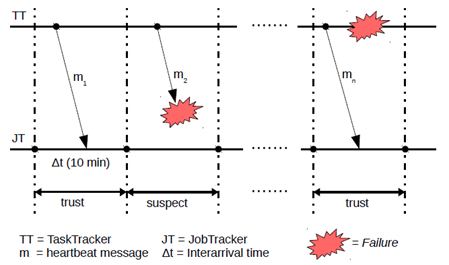
\includegraphics[width=12cm]{./image/tasktracker.png}}
  \caption{TaskTracker Failure Detection Model in Hadoop Framework}\label{fig:tasktracker}
  [From: Adaptive Failure-Aware Scheduling for Hadoop. (Mbarka Soualhia, Montreal, Quebec, Canada, 2018)]
\end{figure}

\hspace{10mm}For example, active TaskTracker send heartbeat messages to JobTracker every 3 seconds.  While JobTracker check the timeout condition every 200 seconds.  There are network delays or messages losses, so some heartbeat may arrive late or loss.  The JobTracker may consider that TaskTracker as dead node even it is available as shown in \textbf{Figure}~\ref{fig:tasktracker}. that heartbeat message m2 does not arrive and the JobTracker consider this TaskTracker as dead.

\newpage

%%% Container Technology
\subsection{Container Technology}

\begin{figure}[!h]\centering
  \setlength{\fboxrule}{0mm} % can define this in the preamble
  \setlength{\fboxsep}{0cm}
  \fbox{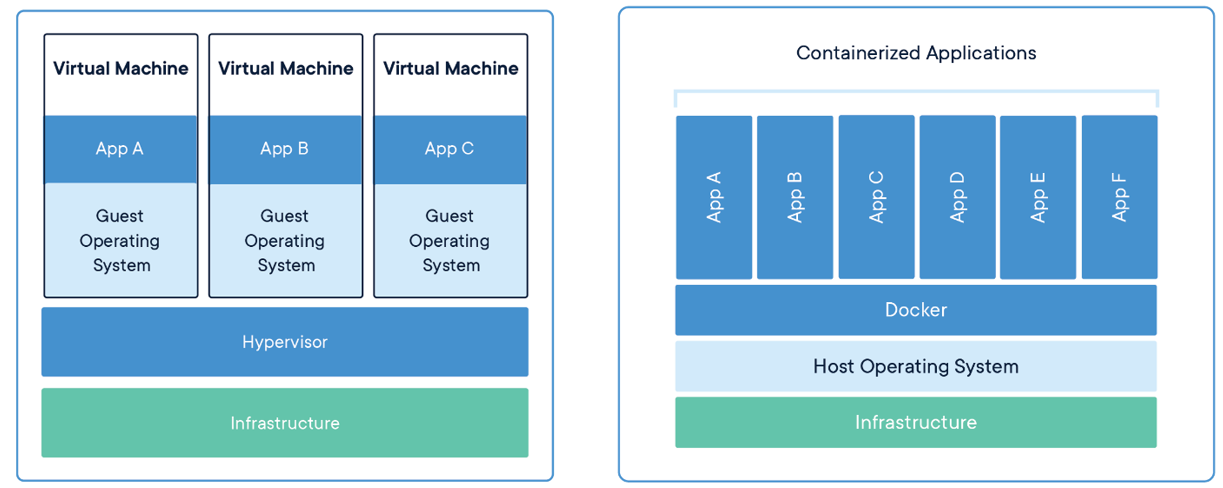
\includegraphics[width=13cm]{./image/vmVSContainer.png}}
  \caption{Virtual machine vs Container}\label{fig:vmVSContainer}
  [From: Docker, "What is a Container?," [Online]. Available: www.docker.com/resources/what-container. Accessed 30 August 2020]
\end{figure}

\hspace{10mm}Container Technology is a method to package up code and all its dependencies, so the application runs quickly and reliably from one computing environment to another, with container software having names including the popular choices of Docker, Apache Mesos, RKT, and Kubernetes.  The virtual machine contains the entire operating system.  Therefore, the physical server that runs several virtual machines is running several operating systems’ simultaneously as shown in \textbf{Figure}~\ref{fig:vmVSContainer}. \cite{docker}

\hspace{10mm}There is a lot of overhead on virtual machine.  In contrast, with container technology, the server runs a single operating system.  Each container can share this single operating system with other containers on server.  Containers require less resource of server with less overhead and more efficient than virtual machines. \cite{container}   Containers are set up to accomplish work in a multiple container architecture (container cluster).  They also enable a program to be broken down into smaller pieces, which are known as microservices.  So, the program can work on each of the containers separately.

%%% Overview of machine learning
\subsection{Overview of machine learning}
\hspace{10mm}Machine learning is a branch of artificial intelligence (AI).  It is the machine’s ability to learn from data provided without human intervention and able to improve decision from experience.  Without human directed programming instructions, the machine accesses data, observes and finds data pattern.  The more data input the better data pattern learning and better decision making.\cite{ml}

%%% AI - Artificial Neural network
\subsection{AI - Artificial Neural network}
\hspace{10mm}An artificial neural network (ANN) is a computational model imitates the natural human brain. The network consists of hundreds or thousands small neuron nodes. Those numerous neuron nodes communicate to each other in the web form. The neuron node is called processing unit. Each of processing unit is interconnected by nodes. Each processing unit comprises of input unit and output unit. Input unit receives various type of data format. It also has an internal weighting system. The neural network learns from the input and produce output result.

\hspace{10mm}ANN use rules and guidelines to generate result/ output. The set of these learning rules is called backpropagation because it uses backward propagation of error to learn or improve the better result. ANN learns data patterns in training phase. It compares actual output with the desired output that is expected result in supervised phase. The difference between actual and expected result are worked backward to adjust the weight of its connections between the units. The purpose is to make the lowest possible error. \cite{ann}

%%% Deep learning
\subsection{Deep learning}
\hspace{10mm}Nowadays, there are collections of vast unlabeled and unstructured data gathering from various sources that is difficult to analyses useful information by traditional programs in a linear way.  The hierarchical level of artificial neural network that work in web form to process data with a nonlinear approach is called Deep Learning.  The first layer of the neural network processes a raw data and pass output on to the next layer. The second layer processes first layer output plus additional information and pass output to next layer again. This continues across all levels of the neuron network to make information more meaningful information. \cite{deepLearning}

\hspace{10mm}Deep learning models can achieve high accuracy, sometimes exceeding human-level performance. “Deep” refers to the powerful number of hidden layers in the neural network.  However, it needs lots of labeled data and high-performance machines to analyze. The organized layers of interconnected nodes can be tens or hundreds of hidden layers. \cite{deepLearning2} as shown in \textbf{Figure}~\ref{fig:NN}.

\begin{figure}[!h]\centering
  \setlength{\fboxrule}{0mm} % can define this in the preamble
  \setlength{\fboxsep}{0cm}
  \fbox{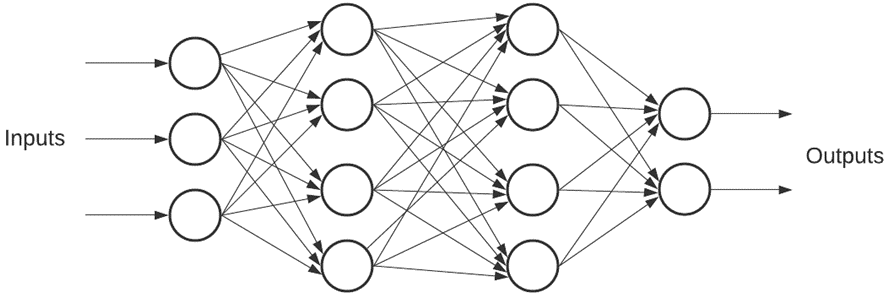
\includegraphics[width=14cm]{./image/NN.png}}
  \caption{Neural networks.}\label{fig:NN}
\end{figure}

\newpage

%%%%%%%%%% Technologies survey %%%%%%%%%%%%
\section{Technologies survey}  

%%% Apache Mesos
\subsection{Apache Mesos}
\hspace{10mm}Mesos consists of a master, agent daemons running on each cluster node, and Mesos frameworks that run task on these agents as shown in \textbf{Figure}~\ref{fig:MesosArc}. Architecture consist of three components: masters, slaves, and the frameworks that run on them. Mesos relies on Apache ZooKeeper, a distributed database used specifically for coordinating leader election within the cluster, and for leader detection by other Mesos masters, slaves, and frameworks. \cite{mesosInAction}

\begin{figure}[!h]\centering
  \setlength{\fboxrule}{0mm} % can define this in the preamble
  \setlength{\fboxsep}{0cm}
  \fbox{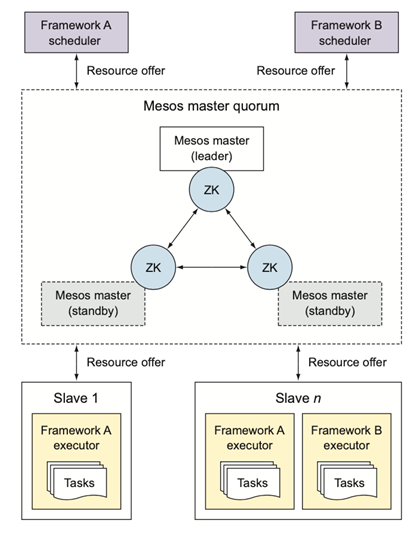
\includegraphics[width=10cm]{./image/MesosArc.png}}
  \caption{The Mesos architecture consists of one or more masters, slaves, and frameworks.}\label{fig:MesosArc}
  [From: Ignazio, R. Mesos in Action (Manning Publications Co., Shelter Island, NY, 2016).]
\end{figure}

\begin{enumerate}
  \item \textbf{Masters: } Mesos masters are responsible for managing the Mesos slave daemons running on each machine in the cluster. Using Zookeeper, they coordinate which node will be the leading master, and which masters will be on standby, and ready to take over if the leading master goes offline. A Mesos cluster requires minimum one master, and three or more are recommended for production deployments. Zookeeper can run on the same machines as the Mesos masters themselves or use a standalone Zookeeper cluster. 
  \newpage
  \item \textbf{Slaves: } The machines in a cluster responsible for executing a framework’s tasks.
  \item \textbf{Frameworks: } Mesos application that’s responsible for scheduling and executing tasks on a cluster. A framework is made up of two components: a scheduler and an executor. 
  \begin{itemize}
      \item \textbf{Schedulers} A scheduler is a long-running service responsible for connecting to a Mesos master and accepting or rejecting resource offers. Mesos delegates the responsibility of scheduling to the framework, instead of attempting to schedule all the work for a cluster itself. The scheduler can then accept or reject a resource offer based on whether it has any tasks to run at the time of the offer. 
      \item \textbf{Executor} An executor is a process launched on a Mesos slave that runs a framework’s tasks on a slave.
  \end{itemize}
\end{enumerate}

\hspace{10mm}Dominant resource is a resource of specific type (CPU, memory, disk, ports) which is most demanded by given framework among other resources it needs. DRF computes the share of resource allocated to a framework (dominant share) and tries to maximize the smallest dominant share in the system. for next round offers the resources first to the one with smallest dominant share, then to the second smallest one and so on. \cite{drf} Example with 9 CPUs and 18 GB RAM to two frameworks running task that require <1 CPU, 4GB> and <3CPUs, 1GB> shown in \textbf{Table}~\ref{tbl:DRFTwoFramework}.

\begin{table}[!h]
  \caption{Example of running 2 frameworks.}\label{tbl:DRFTwoFramework}
  \begin{tabular}{|c|c|c|c|c|c|c|}
    \hline
    \multirow{2}{*}{Schedule} & \multicolumn{2}{c|}{Framework A}& \multicolumn{2}{c|}{Framework B}& \multicolumn{2}{c|}{total}\\ 
    \cline{2-7} & Resource Share & Dominant Share & Resource Share & Dominant Share & CPU & RAM \\ 
    \hline
    B  & <0, 0> & 0 & <3/9, 1/18> & 1/3 & 3/9 & 1/18 \\ 
    \hline
    A  & <1/9>, <4/18> & \textbf{2/9} & <3/9, 1/18> & 1/3 & 4/9 & 5/18 \\ 
    \hline
    A  & <2/9>, <8/18> & 4/9 & <3/9>, <1/18> & \textbf{1/3} & 5/9 & 8/18 \\ 
    \hline
    B  & <2/9>, <8/18> & \textbf{4/9} & <6/9>, 2/18> & 2/3 & 8/9 & 10/18 \\ 
    \hline
    A  & <3/9>, <12/18> & 2/3 & <6/9>, 2/18> & 2/3 & 1 & 14/18 \\ 
    \hline
  \end{tabular}
\end{table}

%%% Zookeeper
\subsection{Zookeeper}
\hspace{10mm}ZooKeeper is an open-source Apache project that provides a centralized service for providing configuration information, naming, synchronization, and group services over large clusters in distributed systems. The goal is to make these systems easier to manage with improved and more reliable propagation of changes. ZooKeeper provides an infrastructure for cross-node synchronization by maintaining status type information in memory on ZooKeeper servers. A ZooKeeper server keeps a copy of the state of the entire system and persists this information in local log files. Large Hadoop clusters are supported by multiple ZooKeeper servers, with a master server synchronizing the top-level servers. \cite{zookeeper}

%%% Elasticsearch
\subsection{Elasticsearch}
\hspace{10mm}Elasticsearch is an open-source search and analytics engine built on Apache Lucene and developed in Java. Elasticsearch can be used to store and search all kinds of documents, analyze huge volumes of data in near real-time and give back answers in milliseconds, and supports multitenancy. It’s able to achieve fast search responses because it searches an index directly instead of searching the text. Related data is often stored in the same index, which consists of one or more primary shards, and zero or more replica shards. Once an index has been created, the number of primary shards cannot be changed. It uses a structure based on documents and comes with extensive REST APIs for storing and searching the data. 

\hspace{10mm}Elasticsearch is the component of the Elastic Stack. Elastic Stack is a set of open-source tools for storage, analysis, and visualization. The four components are Elasticsearch, Logstash, Kibana and Beats. They are designed for use as an integrated solution. It is commonly referred to as the “ELK” stack.\cite{elasticsearch}

%%% Chronos
\subsection{Chronos}
\hspace{10mm}Chronos is the Mesos Cron system. It handles time-based scheduling of jobs on a Mesos cluster. Chronos can be used to schedule commands or scripts. The Chronos feature set is easily and reliably to create standalone schedule-based jobs, as well as complex dependency-based jobs and pipelines, simply by specifying the schedule and resources that the job requires. This guarantees that time-based jobs are running on time while continuing to use datacenter resources as efficiently as possible. In \textbf{Figure}~\ref{fig:chronos}, it shows about the differences between running Cron jobs on a single machine and running them on a Mesos cluster.\cite{mesosInAction}

\begin{figure}[!h]\centering
  \setlength{\fboxrule}{0mm} % can define this in the preamble
  \setlength{\fboxsep}{0cm}
  \fbox{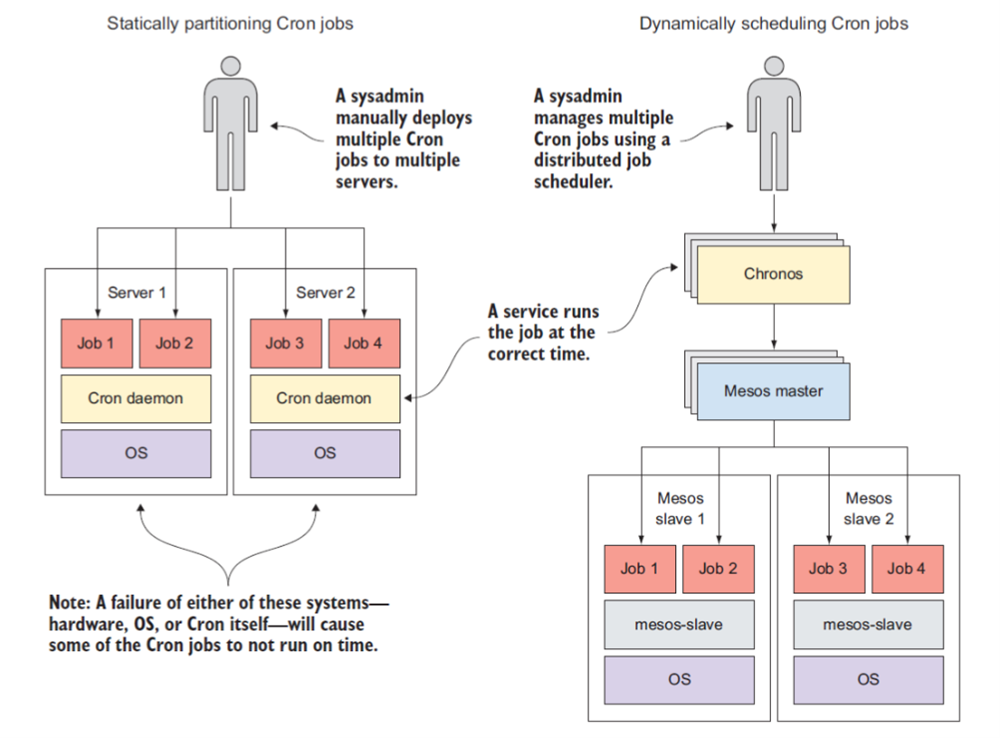
\includegraphics[width=14cm]{./image/chronos.png}}
  \caption{Mesos and Chronos provide a dynamic and fault-tolerant environment to run time-based jobs.}\label{fig:chronos}
  [From: Ignazio, R. Mesos in Action (Manning Publications Co., Shelter Island, NY, 2016).]
\end{figure}

%%% Marathon
\subsection{Marathon}
\hspace{10mm}Marathon is a popular open source Mesos framework developed by Mesosphere. Marathon is used for deploying long-running services and applications, both in Linux cgroups and Docker containers. It can also be considered a private platform as a service (PaaS) on which to deploy applications. Marathon can specify the resources needed for each instance of an application and number of running instances. If a Mesos slave fails, or an instance of application crashes or exits, Marathon will automatically start a new instance to replace the failed one.

\hspace{10mm}Marathon also allows users to specify dependencies on other services and applications during deployment, so an application instance can’t start before its database instance is up and passing health checks. Marathon contains a list of features that should satisfy the needs of most application management scenarios such as managing applications and groups of applications with dependencies and health checks, rolling application upgrades with specific capacity requirements, a powerful web interface and REST API, and high availability (using ZooKeeper for leader election and coordination).\cite{mesosInAction}

%%% Spark
\subsection{Spark}
\hspace{10mm}Apache Spark is unified analytics engine for large-scale data processing. It runs on Hadoop, Apache Mesos, Kubernetes, standalone, or in the cloud. It can access diverse data sources. Spark perform task faster and more efficiently than Hadoop’s MapReduce, both in memory and on disk in many cases. Spark also provide API for several programming language, including Python, Scala, and Java and support streaming workloads, interactive queries and machine learning libraries, in addition to MapReduce-like batch processing.  Spark can run locally. But that is useful only for development purpose, the number of CPU cores limits the number of executors. When setting up a production Spark cluster, there are two option.

\hspace{10mm}When setting up statically partitioned cluster on an Infrastructure as a Service (IaaS) provider. It will be wasting money due to cloud instances sitting idle. Find-grained resource sharing can help increase system’s utilization. For example, if there are two applications likes in \textbf{Figure}~\ref{fig:spark}, Spark and Jenkins that need to run on multiple servers. Each of these system atop a general-purpose cluster manager like Mesos that allows for this sort of fine-grained resource sharing. It can share compute resources and run multiple workloads on a single Mesos slave. This will lead to better resource utilization across many machines within a modern datacenter.\cite{mesosInAction}

\begin{figure}[!h]\centering
  \setlength{\fboxrule}{0mm} % can define this in the preamble
  \setlength{\fboxsep}{0cm}
  \fbox{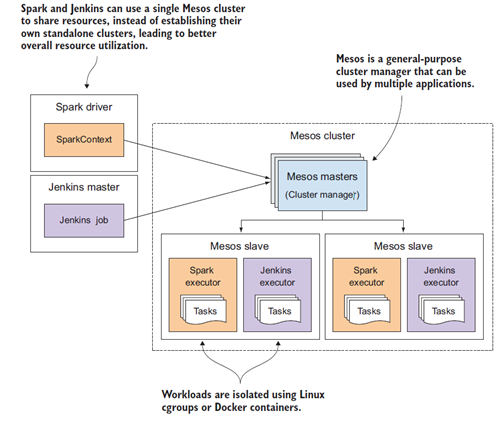
\includegraphics[width=13cm]{./image/spark.png}}
  \caption{Mesos managing cluster resources for two applications.}\label{fig:spark}
  [From: Ignazio, R. Mesos in Action (Manning Publications Co., Shelter Island, NY, 2016).]
\end{figure}

%%% Apache Kafka
\subsection{Apache Kafka}
\hspace{10mm}Apache Kafka is an open-source stream-processing software platform. Apache Kafka is providing a unified, high-throughput, and low-latency platform for handling real-time data feeds. Kafka allows user to subscribe itself and publish data to any number of systems or real-time applications. In \textbf{Figure}~\ref{fig:kafka}, producers are processes that send message to Kafka. Kafka stores these messages in key-value. The data can be partitioned into different topic. Consumers are process that can read messages from partitions. Kafka runs on a cluster of one or more server, And the topics are distributed across the cluster nodes. Partitions are replicated to multiple servers.\cite{kafka}

\begin{figure}[!h]\centering
  \setlength{\fboxrule}{0mm} % can define this in the preamble
  \setlength{\fboxsep}{0cm}
  \fbox{
\includegraphics[width=10cm]{./image/kafka.png}}
  \caption{Overview of Kafka.}\label{fig:kafka}
  [From: wikipedia.''Kafka''.[online].Available:\url{en.wikipedia.org/wiki/Apache_Kafka}.Accessed 25 November 2020]
\end{figure}

%%%%%%%%%% Related Research %%%%%%%%%%%%
\section{Related Research}
\hspace{10mm}The current data center management is a representative large-scale resource management and scheduling framework for clusters, liked the open-source project Mesos \cite{mesosInAction}. However, the data center environment are cluster systems and variety of submitted tasks, such as Hadoop clusters that support big data processing and Spark clusters that support in-memory computing. Mesos is a resource allocation method with no differential task type and scheduler does not consider the overall resource demand or workload, which leads to low average resource utilization and starve were a framework with a high demand on queue. Moreover, Mesos uses the DRF (Dominant Resource Fairness) algorithm for resource allocation. The DRF algorithm is the default scheduling algorithm of Mesos, the algorithm still has the disadvantage of not considering the machine performance and task type.

\hspace{10mm}Many researchers have conducted relevant work. For example, in 2016, Li Y et al \cite{fishSwarm} introduced the fish swarm intelligence algorithm to dynamically adjusting the Mesos cluster resources to improve the Mesos load imbalance and resource utilization. The DRF scheduling algorithm of Mesos is extended, and in 2018, Wenbin Liu et al. proposed A X-DRF algorithm \cite{xdrf} based on building classifies the performance of physical machines and job type judgment classification is proposed to solve the problem of machine performance in literature, but the task type is not considered and not consider the waiting time. Compared with the original DRF algorithm, the X-DRF algorithm has higher system resource utilization rate, which is in line with the actual production rules of data centers, and provides new ideas for heterogeneous cluster multi- resource management for data center managers. In 2019, Pankaj Saha et al. developed Tromino \cite{tromino}, a policy driven queue manager. Tromino allows task from individual frameworks to be scheduled based on each framework’s overall resources requirement and current resources consumption. Tromino reduce the impact of unfairness due to framework specific configuration and unfair waiting time due to higher resource demand in a pending task queue.

%%%%%%%%%%%%%%%%%%%%%%%%%%%%%%%%%%%%%%%%%%%%%%%%%%%%%
%%%%%%%%%%%%%%%%%Methodology and Design%%%%%%%%%%%%%%%%%%%%%%%%
%%%%%%%%%%%%%%%%%%%%%%%%%%%%%%%%%%%%%%%%%%%%%%%%%%%%%
\chapter{Methodology and Design}

\hspace{10mm}This chapter covers how this work designs an architecture of meta-scheduler, how config to simulating and setting, how a policy scheduling a task, how this work designs a model, and how to achieve the hypothesis that needs to answer.

%%%%%%%%%% Project Functionality %%%%%%%%%%%%
\section{Project Functionality}
\hspace{10mm}This project is based on the hypothesis If the dominant share and demand awareness is known by meta-scheduler, the failure job in each framework will be reduced.It aims to design additional architecture (meta-scheduler) of Apache Mesos to prove the hypothesis above. The user submits the task directly to the meta-scheduler. When the meta-scheduler accepts tasks, it aggregates all tasks based on data from cluster master for a better fairness and utilization.

%%% sqquence diagram
\subsection{Sequence diagram} 
\begin{figure}[!h]\centering
  \setlength{\fboxrule}{0mm} % can define this in the preamble
  \setlength{\fboxsep}{0cm}
  \fbox{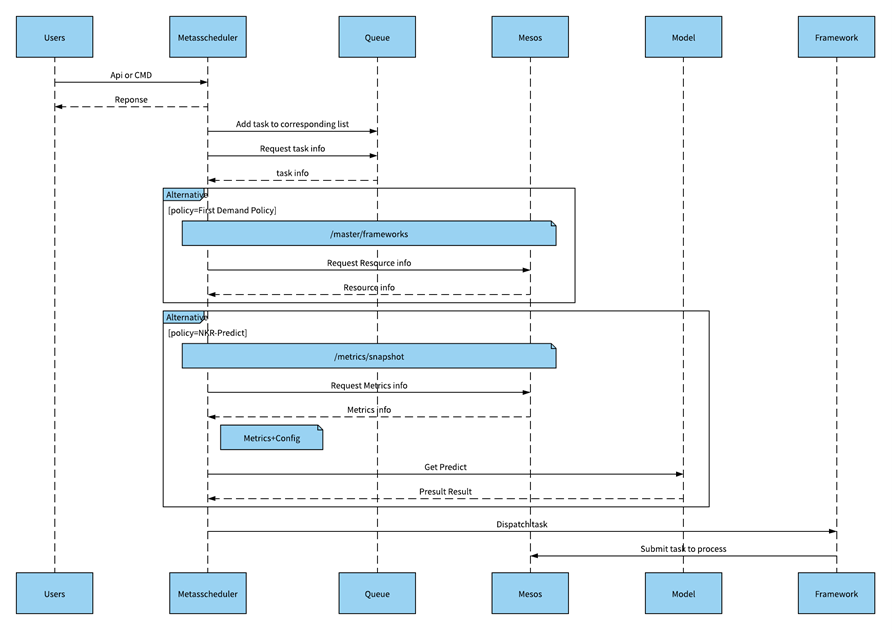
\includegraphics[width=16cm]{./image/SequenceDiagram.png}}
  \caption{Sequence diagram of Apache Mesos}\label{fig:SequenceDiagram}
\end{figure}

\hspace{10mm}\textbf{Figure}~\ref{fig:SequenceDiagram} shows sequence diagram that user submits a job via command line or Application Programming Interface (API), and also specifies their framework, resources requirement, configuration script, and command to the meta-scheduler. The meta-scheduler, called NKR-scheduler, keeps track of incoming task from user and distributes each task to the queue. NKR-scheduler periodically fetches cluster and task information from Mesos Master to make a decision for task scheduling based on pre-defined policy (to be explained in Topic 3.2.2).  After NKR-scheduler finishes a decision-making process, it will dispatch task directly to corresponding framework.

%%% Hypothesis Testing
\subsection{Hypothesis Testing} 
\hspace{10mm}Hypothesis Testing was set up in order to proof that NKR-scheduler can reduce number of failed task and improve fairness in each framework by considering both Dominant share and Demand awareness which describes more detail in \textbf{Table}~\ref{tbl:VariableDescription}. There are three frameworks which are Marathon, Chronos, and Spark for the test. The results were compared using 4 criteria for executing framework;
\begin{enumerate}
  \item \textbf{Normal Cluster Setting}: not using NKR-scheduler 
  \item \textbf{NKR-scheduler}: apply with Policy 1 (First Demand Share Policy)
  \item \textbf{NKR-scheduler}: apply with Policy 2 (Success Rate Prediction)
  \item \textbf{NKR-scheduler}: apply with both Policies (Hybrid Policy)
\end{enumerate}

\begin{table}[!h]
  \caption{Variable description.}\label{tbl:VariableDescription}
  \begin{tabular}{@{}|p{0.2\textwidth}|p{0.8\textwidth}|}
    \hline
    \textbf{Variable} & \textbf{Description}\\
    \hline
    \textbf{Dominant share} & The resource that each framework uses in cluster at that point of time\\
    \hline
    \textbf{Demand awareness} & resource requirement of each framework \\
    \hline
  \end{tabular}
\end{table}

\textbf{Experiment:} Frameworks with same arrival rate and all tasks are vary in a resource consumption as shown in \textbf{Table}~\ref{tbl:Experiment}. This experiment will run 3 times consist of 1) First Demand Share Policy, 2) Success rate prediction, and 3) Hybrid Policy.

\begin{table}[!h]
  \caption{Variable description.}\label{tbl:Experiment}
  \begin{tabular}{@{}|p{0.2\textwidth}|p{0.4\textwidth}|p{0.4\textwidth}|}
    \hline
    & \textbf{Number os tasks} & \textbf{Arrival rate (sec)}\\
    \hline
    \textbf{Marathon} & 33 & 2\\
    \hline
    \textbf{Chronos} & 33 & 2 \\
    \hline
    \textbf{Spark} & 33 & 2 \\
    \hline
\end{tabular}
\end{table}

\hspace{10mm}The evaluation metrics are 
\begin{enumerate}
  \item \textbf{Improving of fariness:} It is evaluated by Average different task number of each framework. Lower different number is better fairness among frameworks.The formular to it is  shown in \textbf{Table}~\ref{tbl:formular}
    \begin{table}[!h]
    \caption{Parameter Formula and Description.}\label{tbl:formular}
    \begin{tabular}{@{}|p{0.5\textwidth}|p{0.5\textwidth}|}
      \hline
      \textbf{Formula} & \textbf{Description} \\ 
      \hline
      \multirow{3}{*}{$fairness = \frac{|t_m-t_c|+|t_m-t_s|+|t_c-t_s|}{3} $} & $t_m$ average number of Marathon task\\ 
      & $t_c$ average number of Chronos task\\ 
      & $t_s$ average number of Spark task\\ 
      \hline
    \end{tabular}
  \end{table}
  \item \textbf{Reduction of failed tasks:} It is evaluated by number of failed tasks.
  \item \textbf{Additional:} CPU and memory utilization, number of processes were waiting for the CPU (system load), and running time of each frameworks.
\end{enumerate}

\newpage
%%%%%%%%%% System Architecture %%%%%%%%%%%%
\section{System Architecture}

%%%Architecture diagram
\subsection{Architecture diagram}  

\begin{figure}[!h]\centering
  \setlength{\fboxrule}{0mm} % can define this in the preamble
  \setlength{\fboxsep}{0cm}
  \fbox{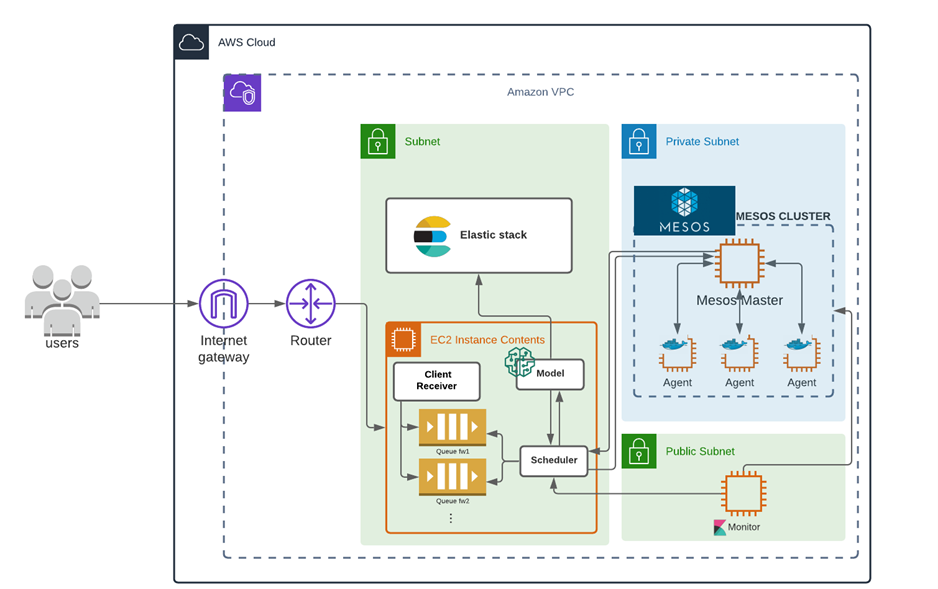
\includegraphics[width=16cm]{./image/ArchitectureDiagram.png}}
  \caption{Architecture diagram.}\label{fig:ArchitectureDiagram}
\end{figure}

\hspace{10mm}According to \textbf{Figure}~\ref{fig:ArchitectureDiagram} shows architecture diagram, there are many components that this project implements. NKR-scheduler consists of three major  components 1) Client Receiver, 2) Queue, and 3) Scheduler and the other components describe below in \textbf{Table}~\ref{tbl:ArchitectureDiagramTable}.

\begin{table}[!h]
  \caption{Description of Architecture diagram.}\label{tbl:ArchitectureDiagramTable}
  \begin{tabular}{@{}|p{0.2\textwidth}|p{0.8\textwidth}|}
    \hline
    \textbf{Components} & \textbf{Description}\\
    \hline
    \textbf{Client Receiver} & Interface for user to submit task to cluster.\\
    \hline
    \textbf{Queue} & The list that stores task and information about resources requirement in each framework that register into the Apache Mesos.\\
    \hline
    \textbf{Scheduler} & The adaptive policy that configured by user and keeps track information about cluster from Apache Mesos.\\
    \hline
    \textbf{Elasticsearch} & Elasticsearch stores previous data from Apache Mesos and periodically train a new model.\\
    \hline
    \textbf{Monitor} & Monitor keeps track abnormality and another metrics.\\
    \hline
    \textbf{Model} & It stores model for predicting in case user want to use AI to schedule tasks.\\
    \hline
  \end{tabular}
\end{table}

\newpage
%%%Policy
\subsection{Policy}  
\hspace{10mm}This project designs two policies for the Meta-scheduler: 1) First Demand Policy (FDP), and 2) Success rate prediction. These policies can be extended further based on scheduling needs of users. 

%%%%% 1.FDP
\begin{enumerate}
  \item \textbf{First Demand Share Policy} We explain how FDP policy work by considering, a cluster with a total of 8 CPU and 64 GB of memory, where two frameworks (A and B) are shared completely shared resources. Each framework can have different number of tasks in its list. In example, framework a has 4 tasks each task consumes (2 CPU, 0.5GB memory) as a resource demand, and Framework B has 2 tasks with (0.5 CPU, 1 GB memory) and task still running on cluster. Framework A has 1 task (2CPU, 0.5 GB memory), and Framework B has 2 task (1CPU, 2 GB memory) the dominants share of framework A = max (2/8,0.5/64) = 25\% and Framework B = 12.5\%. In this case if we apply normal scheduling policy it will dispatch task from framework B as shows in \textbf{Figure}~\ref{fig:flowDiagram}.

  \begin{figure}[!h]\centering
    \setlength{\fboxrule}{0mm} % can define this in the preamble
    \setlength{\fboxsep}{0cm}
    \fbox{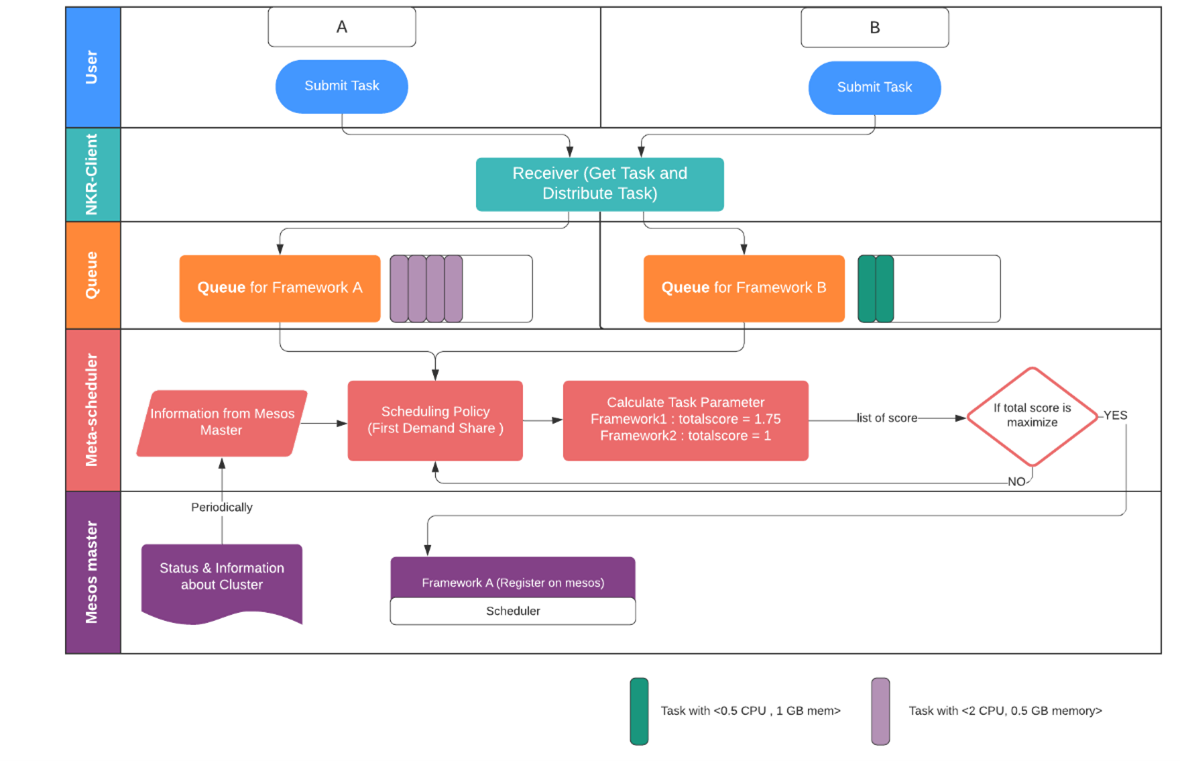
\includegraphics[width=15cm]{./image/flowDiagram.png}}
    \caption{Architecture diagram.}\label{fig:flowDiagram}
  \end{figure}

\hspace{10mm}In FDP policy, we consider both the demands of each framework and their dominant share that come from cluster monitor. Scheduling only based on the demand may cause unfairness. A framework could end up consuming the entire cluster due to its higher demand while another framework that has significantly fewer number of tasks to execute could starve for resources. Therefore, we combine both as a factor and use decision matrix in each cycle to decide which task to be dispatched. We present how to calculate each parameter in \textbf{Table}~\ref{tbl:Parameter}. according to \textbf{Table}~\ref{tbl:DecisionMatrix}, We can see highly total factor in framework A, therefore program assign a higher priority and let its corresponding dispatcher release a task

  \begin{table}[!h]
    \caption{Parameter Formula and Description.}\label{tbl:Parameter}
    \begin{tabular}{@{}|p{0.3\textwidth}|p{0.3\textwidth}|p{0.3\textwidth}|}
      \hline
      \textbf{Parameter name} & \textbf{Formula} & \textbf{Description} \\ 
      \hline
      \multirow{4}{*}{\textbf{Demand Dominant (DD)}} & \multirow{4}{*}{$DD_i = \max_{j=1}^{m}(\frac{n_ird_{i,j}}{r_j})$} & $m$ available types of resources\\ 
      \cline{3-3} & & $n_i$ number of tasks on list $i$\\ 
      \cline{3-3} & & $rd_{i,j}$ resource demand of type j being demand by framework $rd_i $\\ 
      \cline{3-3} & & $r_j$ total resource of type $j$\\ 
      \hline
      \multirow{3}{*}{\textbf{Demand Share (DS)}} & \multirow{3}{*}{$DS_i = \max_{j=1}^{m}(\frac{n_i}{r_j})$} & $m$ available types of resources \\ 
      \cline{3-3} & & $n_i$ number of tasks on list $i$ \\
      \cline{3-3} & & $r_j$ total resource of type $j$ \\ 
      \hline
    \end{tabular}
  \end{table}

  \begin{table}[!h]
    \caption{Decision Matrix.}\label{tbl:DecisionMatrix}
      \begin{tabular}{@{}|p{0.2\textwidth}|p{0.2\textwidth}|p{0.2\textwidth}|p{0.3\textwidth}|}
      \hline
      \textbf{Framework} & \textbf{DD} & \textbf{(1-DS)} & \textbf{TOTAL}\\
      \hline
      \textbf{A} & 1 & 0.75 & 1.75\\
      \hline
      \textbf{B} & 0.125 & 0.875 & 1\\
      \hline
    \end{tabular}
  \end{table}
  
  \newpage
%%%%% 2.Success rate prediction
  \item \textbf{Success rate prediction}There are many metrics in this policy that affect system or task performance, such as CPU utilization, free memory, storage in use, message send information, message queue length, average execution time, and etc. These metrics are able to identify anomalies (task failed, task killed, and etc.) by using the pipeline provided in \textbf{Topic} 3.3.2
  
\hspace{10mm}Firstly, the log data need to be pre-processed by transforming and cleaning.  Secondly, the log data are clustered by K-means algorithm to separate the data that point into different metric groups or different machines.  The success rate prediction of given task will use the Random Forest. Random Forest is a set of interconnected decision tree that uses the majority voting to provide classification or regression result. It is robust to noise and able to provide highly accurate prediction. \cite{adaptiveScheduling} In each cluster, the model will be trained by active and terminated tasks information. 

\hspace{10mm}In each cluster, data will be divided into 80\% training dataset and remaining 20\% testing dataset. The measure metric is accuracy, precision, recall ,and error. When users submit task, NKR-scheduler will request metric information from Mesos, allocate resource to run tasks, profile the task to data cluster and use that cluster model to predict success rates of their task shown in \textbf{Figure}~\ref{fig:flowDiagramPredict}.

  \begin{figure}[!h]\centering
    \setlength{\fboxrule}{0mm} % can define this in the preamble
    \setlength{\fboxsep}{0cm}
    \fbox{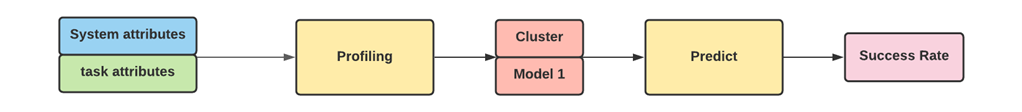
\includegraphics[width=16cm]{./image/flowDiagramPredict.png}}
    \caption{Flow Diagram of Predicting success rate.}\label{fig:flowDiagramPredict}
  \end{figure}

\end{enumerate}

\newpage
%%%Database Schema
\subsection{Database Schema}  

\hspace{10mm}This project implement database as a Elasticsearch and keep log every minute. It allows storing, searching, and analyzing big volumes of data quickly and schema-less. It uses a default configuration to index the data. Database schema shows in \textbf{Figure}~\ref{fig:database} and describe each field in \textbf{Table}~\ref{tbl:fieldName}

\begin{figure}[!h]\centering
  \setlength{\fboxrule}{0mm} % can define this in the preamble
  \setlength{\fboxsep}{0cm}
  \fbox{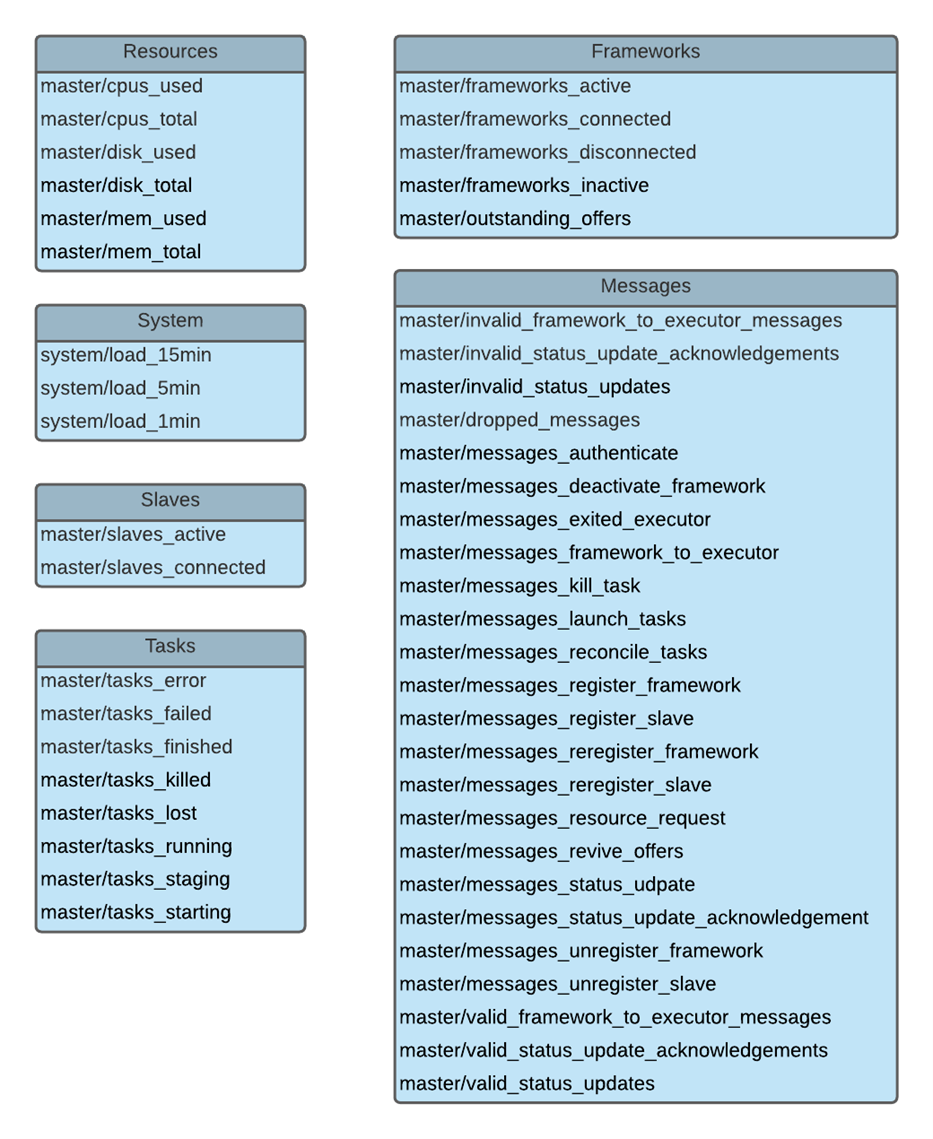
\includegraphics[width=13cm]{./image/database.png}}
  \caption{database schema.}\label{fig:database}
\end{figure}

\begin{table}[!h]
  \caption{Field name and description.}\label{tbl:fieldName}
    \begin{tabular}{|p{0.2\textwidth}|p{0.15\textwidth}|p{0.15\textwidth}|p{0.4\textwidth}|}
    \hline
    \textbf{Index Name} & \multicolumn{3}{p{0.7\textwidth}|}{\textbf{Description}}  \\ 
    \hline
    \textbf{Resources index} & \multicolumn{3}{p{0.7\textwidth}|}{ The following metrics provide information about the total resources available in the cluster and their current usage.} \\ 
    \hline
    \multirow{5}{*}{\textbf{System index}} & \multicolumn{3}{p{0.7\textwidth}|}{ The following metrics provide information about the resources available on this master node and their current usage.} \\ 
    \cline{2-4} & \textbf{Field name} & \textbf{Data type} & \textbf{Description} \\ 
    \cline{2-4} & Load\_15min & Double & Load average for the past 15 minutes \\ 
    \cline{2-4} & Load\_5min & Double & Load average for the past 5 minutes \\ 
    \cline{2-4} & Load\_1min & Double & Load average for the past 1 minutes \\ 
    \hline
    \textbf{Slave index} & \multicolumn{3}{p{0.7\textwidth}|}{ The following metrics provide information about slave events, slave counts, and slave states.} \\ 
    \hline
    \multirow{5}{*}{\textbf{Task index}} & \multicolumn{3}{p{0.7\textwidth}|}{ The following metrics provide information about active and terminated tasks. A high rate of lost tasks may indicate that there is a problem with the cluster.} \\ 
    \cline{2-4} & \textbf{Field name} & \textbf{Data type} & \textbf{Description} \\ 
    \cline{2-4} & tasks\_error & Double & Number of tasks that were invalid \\ 
    \cline{2-4} & tasks\_failed & Double & Number of failed tasks \\ 
    \cline{2-4} & tasks\_finished & Double & Number of finished tasks \\ 
    \cline{2-4} & tasks\_killed & Double & Number of killed tasks \\ 
    \cline{2-4} & tasks\_lost & Double & Number of lost tasks \\ 
    \cline{2-4} & tasks\_running & Double & Number of running tasks \\ 
    \cline{2-4} & tasks\_staging & Double & Number of staging tasks \\ 
    \cline{2-4} & tasks\_starting & Double & Number of starting tasks \\ 
    \hline
    \textbf{Framework index} & \multicolumn{3}{p{0.7\textwidth}|}{ The following metrics provide information about the registered frameworks in the cluster.} \\ 
    \hline
    \textbf{Message index} & \multicolumn{3}{p{0.7\textwidth}|}{ The following metrics provide information about messages between the master and the slaves and between the framework and the executors. A high rate of dropped messages may indicate that there is a problem with the network.} \\ 
    \hline
  \end{tabular}
\end{table}

\newpage

%%%%%%%%%% Data management %%%%%%%%%%%%
\section{Data management}

\subsection{Which dataset is use for training?}
\hspace{10mm}The dataset is created by simulating frameworks that commonly use for Mesos cluster. The types of framework is devided into 3 types 1) Application management and batch scheduling, 2) Data processing, and 3) Distributed databases and storage. it will cover only 2 types of framework. This project implements a job simulator to submit frameworks that work well with Apache Mesos and used by many organizations. Nowadays, the simulator simulates based on following example typically job, shown in \textbf{Table}~\ref{tbl:MesosFramework} and the application job will run according to \textbf{Table}~\ref{tbl:ApplicationData} for one week, and the minimum task for a day is 50 for each framework.

\begin{table}[!h]
  \caption{Framework of Apache Mesos.}\label{tbl:MesosFramework}
    \begin{tabular}{@{}|p{0.45\textwidth}|p{0.15\textwidth}|p{0.15\textwidth}|p{0.15\textwidth}|}
    \hline
    \textbf{Type of Framework} & \textbf{Framework1} & \textbf{Framework2} & \textbf{Framework3}\\
    \hline
    1. Application management and batch scheduling & Chronos & Marathon & \\
    \hline
    2. Data processing &  & & Spark\\
    \hline
  \end{tabular}
\end{table}

\begin{table}[!h]
  \caption{Application Data.}\label{tbl:ApplicationData}
    \begin{tabular}{@{}|p{0.2\textwidth}|p{0.7\textwidth}|}
    \hline
    \textbf{Framework} & \textbf{Application job}\\
    \hline
    Chronos & Wordcount, Kmeans, Topk, and InvertedIndex\\
    \hline
    \multirow{2}{*}{Marathon} & Inline Shell Script and Docker based Application \\
    & https://mesosphere.github.io/marathon/docs/application-basics.html\\
    \hline
    \multirow{2}{*}{Spark} & Wordcount, Pi Estimation, and Text search\\
    & http://spark.apache.org/examples.html\\
    \hline
  \end{tabular}
\end{table}

\newpage

\subsection{Transform data pipeline}

\begin{figure}[!h]\centering
  \setlength{\fboxrule}{0mm} % can define this in the preamble
  \setlength{\fboxsep}{0cm}
  \fbox{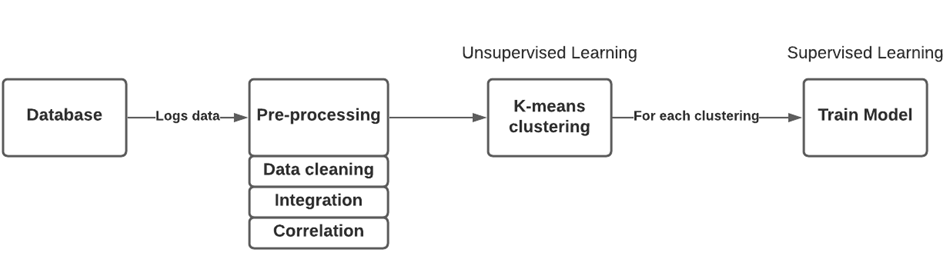
\includegraphics[width=15cm]{./image/dataPipeline.png}}
  \caption{Data pipeline.}\label{fig:dataPipeline}
\end{figure}

This project uses log data that mentioned before to build models by using the following steps below.

\begin{enumerate}
  \item \textbf{Database} Collecting logs data and sending out all of data from last week.
  \item \textbf{Pre-processing}
    \begin{itemize}
      \item \textbf{Data cleaning } Delete uncompleted and unused data. 
      \item \textbf{Integration } Summarizing resource utilization of task, and server.
      \item \textbf{Normalization } Changing value of data into the same range, without distorting differences in the ranges of values.
      \item \textbf{Data selection with correlation } Finding correlation of each attribute and selecting high correlation to build a model.
    \end{itemize}
  \item \textbf{Data Mining } There is plenty of data and we cannot see their relationship, so this project plugs them all into K-means clustering algorithm. It will find data patterns by grouping the data into clusters. We assumed that each cluster is pointed to be a subset of the same machines, task, or framework. Each data cluster will be further investigating. Trhe data will be input those same metrics into the machine learning model.
\end{enumerate}
%%%%%%%%%%%%%%%%%%%%%%%%%%%%%%%%%%%%%%%%%%%%%%%%%%%%%%%%%%%%%%
%%%%%%%%%%%%%%%%%%%% Experiments %%%%%%%%%%%%%%%%%%%%%%%%%%%%%
%%%%%%%%%%%%%%%%%%%%%%%%%%%%%%%%%%%%%%%%%%%%%%%%%%%%%%%%%%%%%%%
\chapter{Experimental setup and results}

\hspace{10mm} In this chapter details about experimental setup that are the control variables in cluster for this experiment, results of simulated data, model for predict success rate ,and result from test run on each policy.

%%%%%%%%%% Setup cluster, framework application, and parameter %%%%%%%%%%%%
\section{Setup cluster, framework application, and parameter}
\hspace{10mm}For the experiment setup, cluster had setup inside a cloud provider which called Amazon Web Services (AWS). This cluster consists of 3 nodes with 2 CPUs, 2.8 GB of memory, and 45 GB of disk for each node as shown in \textbf{Figure}~\ref{fig:resourcesCluster}. This cluster was setup with 3 widely known framework: Mesos, Spark Marathon, and Chronos. The tests were conducted by simulated data with randomly varied resources of each task based on task characteristics. 

\begin{figure}[!h]\centering
    \setlength{\fboxrule}{0mm} % can define this in the preamble
    \setlength{\fboxsep}{0cm}
    \fbox{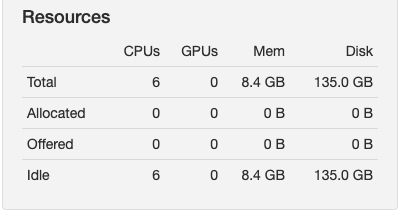
\includegraphics[width=10cm]{./image/resourcesCluster.png}}
    \caption{Resources of the cluster}\label{fig:resourcesCluster}
\end{figure}

Simulated data was created by running sample jobs in a cluster following in \textbf{Table}~\ref{tbl:SimulatedTaskConfiguration}.

\begin{table}[!h]
  \caption{Simulated task configuration.}\label{tbl:SimulatedTaskConfiguration}
  \begin{tabular}{@{}|p{0.2\textwidth}|p{0.3\textwidth}|p{0.4\textwidth}|}
    \hline
    \textbf{Framework} & \textbf{Number of tasks} & \textbf{Arrival Rate (sec)} \\
    \hline
    Marathon & 33 & 2 \\
    \hline
    Chronos & 33 & 2 \\ 
    \hline
    Spark & 33 & 2\\
    \hline                          
  \end{tabular}
\end{table}

\hspace{10mm}From \textbf{Table}~\ref{tbl:SimulatedTaskConfiguration} show the number of tasks running in system to perform simulated task. The details about simulated task in each framework. Firstly, Spark consists of tasks that are implemented in Python-based. There are 2 basic tasks that use to query database and perform left and right join. Secondly, Chronos and marathons have 3 types of tasks running in this system. All tasks consist of vary workload from minimum workload of text classification to maximum workload of training model and genetic algorithm. The result of submitted task is shown in \textbf{Figure}~\ref{fig:task0}.

\begin{figure}[!h]\centering
    \setlength{\fboxrule}{0mm} % can define this in the preamble
    \setlength{\fboxsep}{0cm}
    \fbox{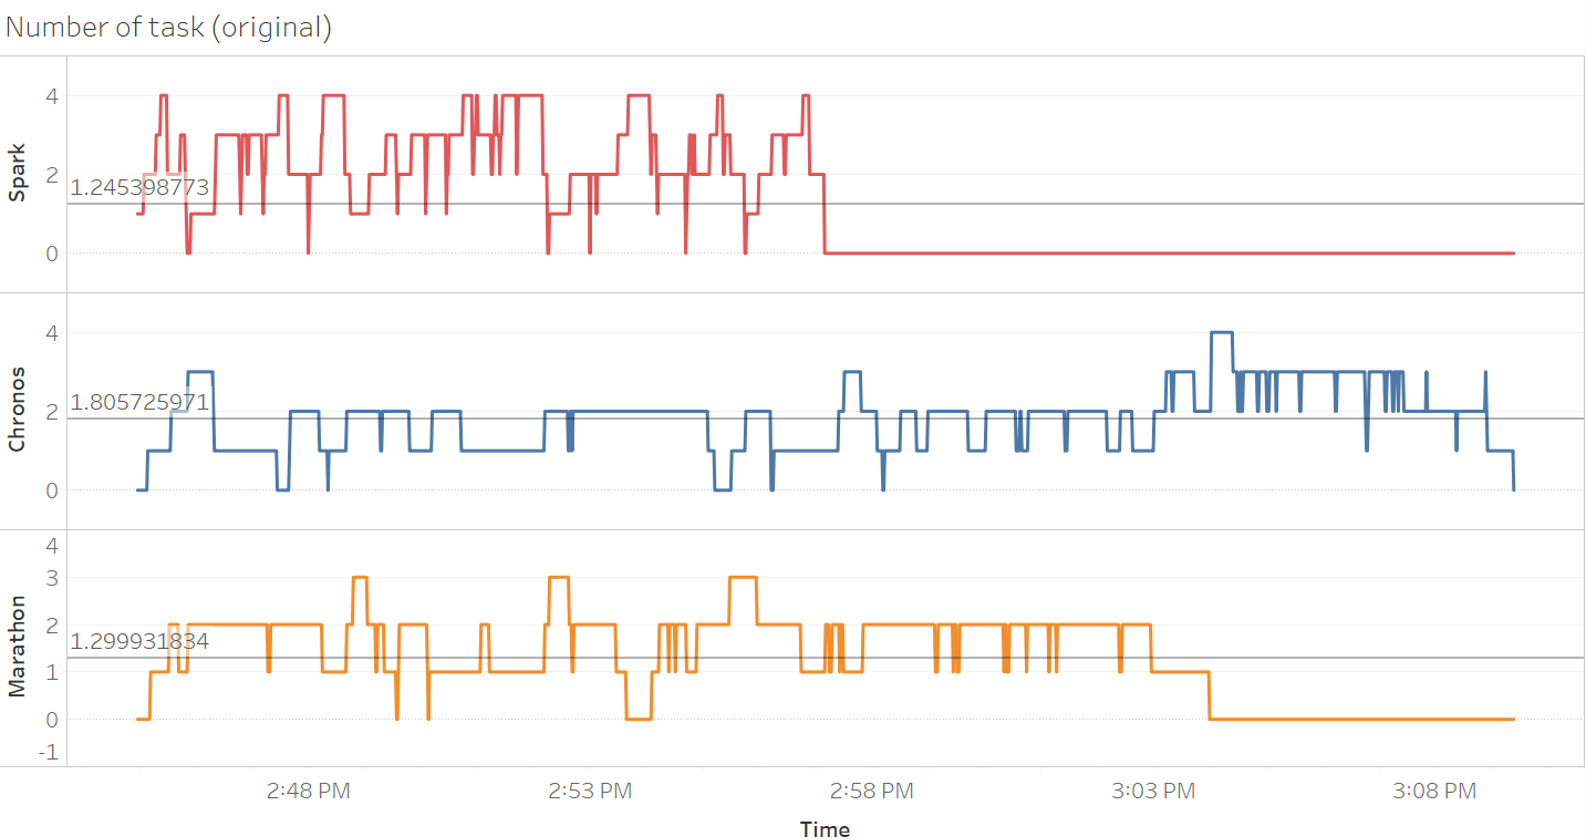
\includegraphics[width=14cm]{./image/chap4/task0.png}}
    \caption{Number of tasks for each framework}\label{fig:task0}
\end{figure}

\newpage

\hspace{10mm}This project got the example of cluster metric data after running sample job in cluster and gathering cluster metric data as shown in \textbf{Figure}~\ref{fig:exampleData}. Each row of cluster metric data was captured every 5 seconds, and each column of cluster metric data was an information of cluster, for example, CPU utilization, memory utilization, number of finished tasks, number of failed tasks, and other information.
\begin{figure}[!h]\centering
    \setlength{\fboxrule}{0mm} % can define this in the preamble
    \setlength{\fboxsep}{0cm}
    \fbox{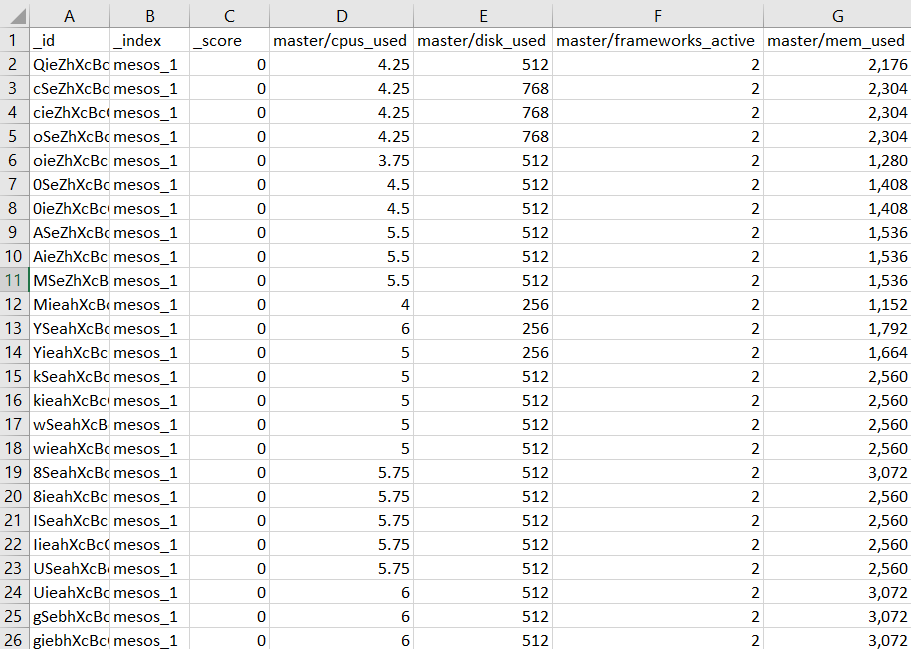
\includegraphics[width=10cm]{./image/exampleData.png}}
    \caption{Example of cluster metric data}\label{fig:exampleData}
\end{figure}

\newpage

%%%%%%%%%% Model for predict success rate %%%%%%%%%%%%
\section{Model for predict success rate}
\subsection{Clustering}  
\hspace{10mm}The metric data was clustered by using k-means algorithm and used elbow method to find optimal k parameter which is number of data cluster in k-means. The result is shown in \textbf{Figure}~\ref{fig:elbow}. From the graph, k = 2 was chosen because at this point the distortion start to decrease in linear form. Therefore, the cluster metric data was separated into 2 clusters by k-means. After separated data into 2 clusters, it was expected that each cluster will be separated by resource utilization. But the result show that resource utilization cannot indicate the cluster they belong to as shown in \textbf{Figure}~\ref{fig:cluster}. 
\begin{figure}[!h]\centering
    \setlength{\fboxrule}{0mm} % can define this in the preamble
    \setlength{\fboxsep}{0cm}
    \fbox{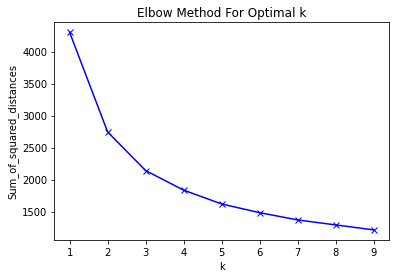
\includegraphics[width=8cm]{./image/elbow.png}}
    \caption{Elbow method for optimal k}\label{fig:elbow}
\end{figure}
\begin{figure}[!h]\centering
    \setlength{\fboxrule}{0mm} % can define this in the preamble
    \setlength{\fboxsep}{0cm}
    \fbox{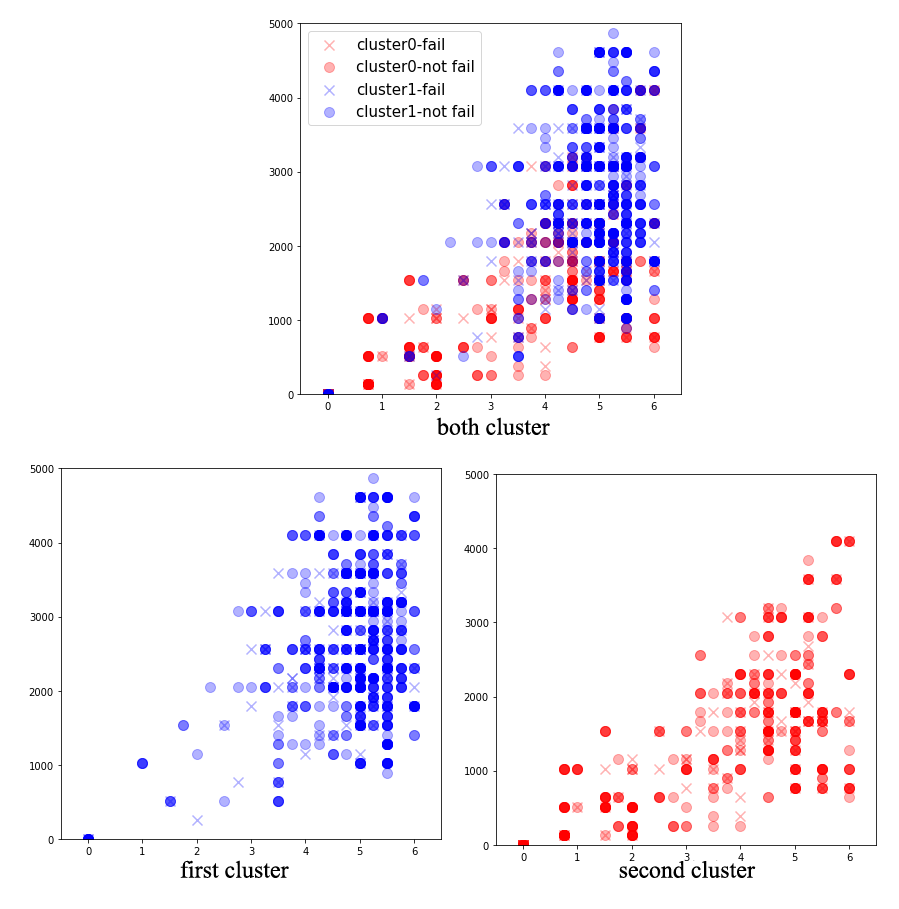
\includegraphics[width=11cm]{./image/cluster.png}}
    \caption{Data clustering visualize by CPU and memory utilization}\label{fig:cluster}
\end{figure}

\newpage

\hspace{10mm}After searching for the characteristic of each cluster and plotting graph as shown in \textbf{Figure}~\ref{fig:highcorr}, It was found that data were clustered by the time that is not applicable to predict success rate. About the correlation of all metrices to the number of fail tasks, the metrices that have high correlation are related to time, and the metrices that have low correlation are either constant or little change over time as shown in \textbf{Figure}~\ref{fig:lowcorr}.
\begin{figure}[!h]\centering
    \setlength{\fboxrule}{0mm} % can define this in the preamble
    \setlength{\fboxsep}{0cm}
    \fbox{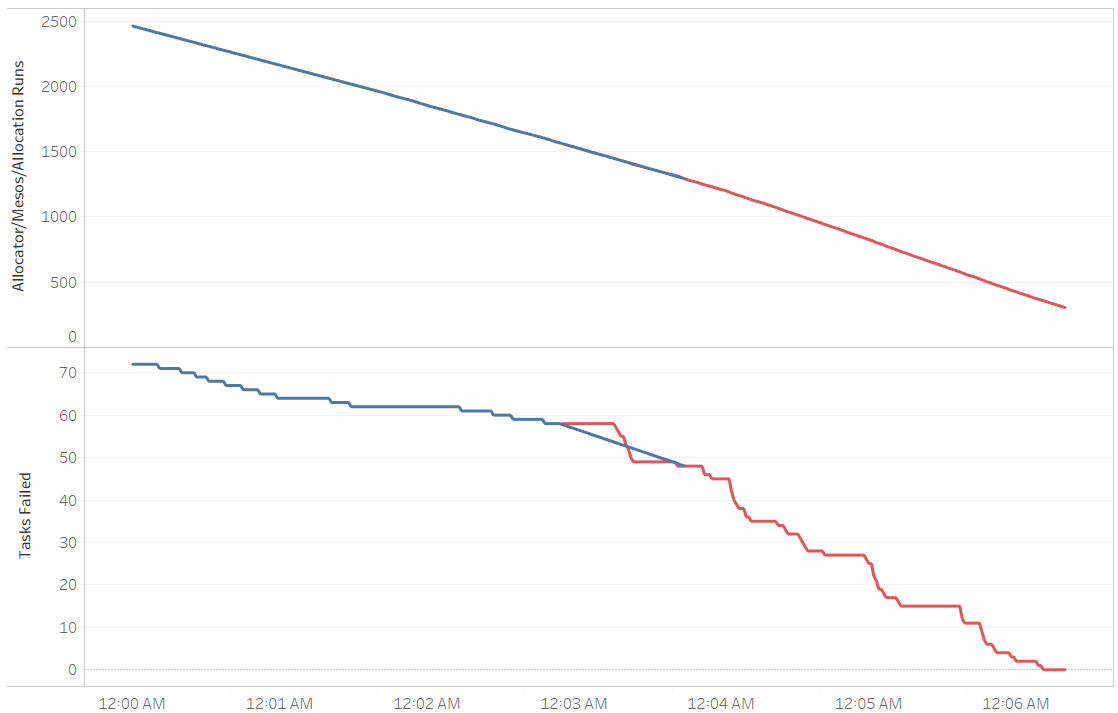
\includegraphics[width=14cm]{./image/highcorr.png}}
    \caption{Data clustering visualize by metrices that have high correlation}\label{fig:highcorr}
\end{figure}
\begin{figure}[!h]\centering
    \setlength{\fboxrule}{0mm} % can define this in the preamble
    \setlength{\fboxsep}{0cm}
    \fbox{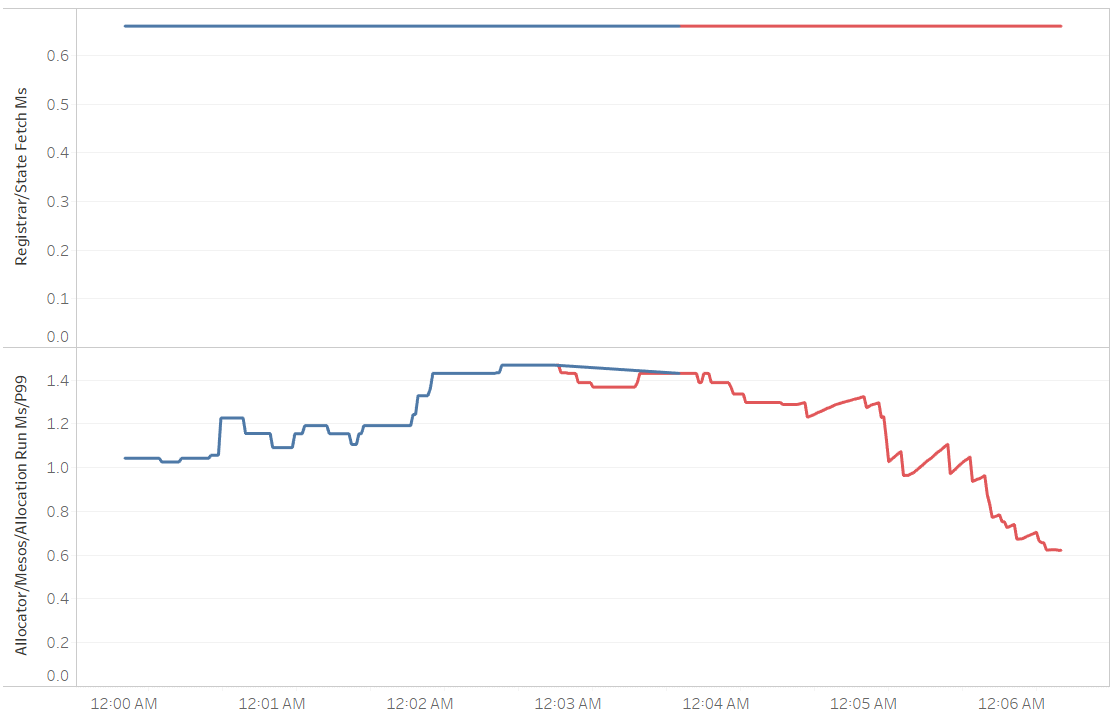
\includegraphics[width=14cm]{./image/lowcorr.png}}
    \caption{Data clustering visualize by metrices that have low correlation}\label{fig:lowcorr}
\end{figure}

%%%%%%%%%% Random forest model %%%%%%%%%%%%
\subsection{Random forest model}  
\hspace{10mm}Random forest model was trained with these following parameters: 
\begin{enumerate}
  \item \textbf{max\_dept}: The maximum dept of the tree sets to be 10
  \item \textbf{random\_stat}: This parameter control randomness of the bootstrapping of the samples used when building tree. 10 is seed for generate random number. Using an integer will produce the same result across different calls. It is easier to check that the results are stable across a number of different distinct random seeds.
  \item \textbf{ma\_features}: For each split, it will consider maximum 10 features.
\end{enumerate}
\hspace{10mm}The result of random forest model is shown in \textbf{Table}~\ref{tbl:RandomForestConfusion}. The accuracy of this model is 0.832, precision is 0.85 and recall is 0.98.

\begin{table}[!h]
  \caption{Result from random forest model.}\label{tbl:RandomForestConfusion}
  \begin{tabular}{@{}|p{0.2\textwidth}|p{0.35\textwidth}|p{0.35\textwidth}|}
   \hline
   \textbf{} & \textbf{Fail (predicted)} & \textbf{Finish (predicted)} \\ 
   \hline
   \textbf{Fail (actuated)} & 317 & 6 \\ 
   \hline
   \textbf{Finish (actuated)} & 58 & 0 \\ 
   \hline                     
  \end{tabular}
\end{table}

%%%%%%%%%% Policy 1: First Demand Share Policy (FDP) %%%%%%%%%%%%
\section{Policy 1: First Demand Share Policy (FDP)}  
\hspace{10mm}FDP used the same setup as mentioned in \textbf{Section 4.1} and use the same submitted tasks in \textbf{Table}~\ref{tbl:SimulatedTaskConfiguration}. NKR-scheduler has developed to receive tasks, and then considers based on the first policy. 

\begin{figure}[!h]\centering
    \setlength{\fboxrule}{0mm} % can define this in the preamble
    \setlength{\fboxsep}{0cm}
    \fbox{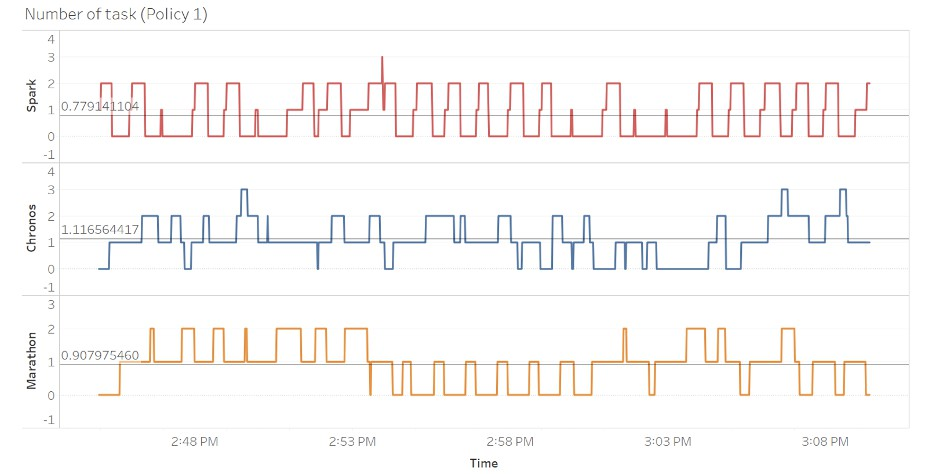
\includegraphics[width=14cm]{./image/chap4/task1.png}}
    \caption{Number of tasks for each framework after using FDP}\label{fig:task1}
\end{figure}

\hspace{10mm}From \textbf{Figure}~\ref{fig:task0}, Marathon and Chronos could not launch a fair number of tasks because Spark could hold on to offer more than the others. After comparing with normal Mesos, there is a little improvement in fairness as shown in \textbf{Figure}~\ref{fig:task1}. Each framework had almost the same approximate number of tasks, which is 1 task. The values that use to compare between before and after applied first policy was following with these values (0.77914, 1.1656, and 0.90797). After calculating the average of difference, the result is 0.257. So, this policy can improve fairness compared to the default policy 0.3736. The result is increased by 31.2\%
\newline
This project also considered these other matrices after applying this policy: 
\begin{enumerate}
%%% po1 fail task
  \item \textbf{Failed task}
  \newline
The result of finished and failed tasks for each framework before and after applied this policy is shown in \textbf{Figure}~\ref{fig:finfail0-1}. The orange color shows percent of finished tasks and the blue one shows percent of failed tasks. The number of Chronos failed tasks was increased, but the number of Marathon and Spark failed tasks was the same. In \textbf{Figure}~\ref{fig:fail1} shows that growth rate of failed tasks is upward when used this policy. The slope was increased from 0.258 to 0.265. So, this policy not only cannot reduce the number of failed tasks but also increase its failure rate.
  \begin{figure}[!h]\centering
    \setlength{\fboxrule}{0mm} % can define this in the preamble
    \setlength{\fboxsep}{0cm}
    \fbox{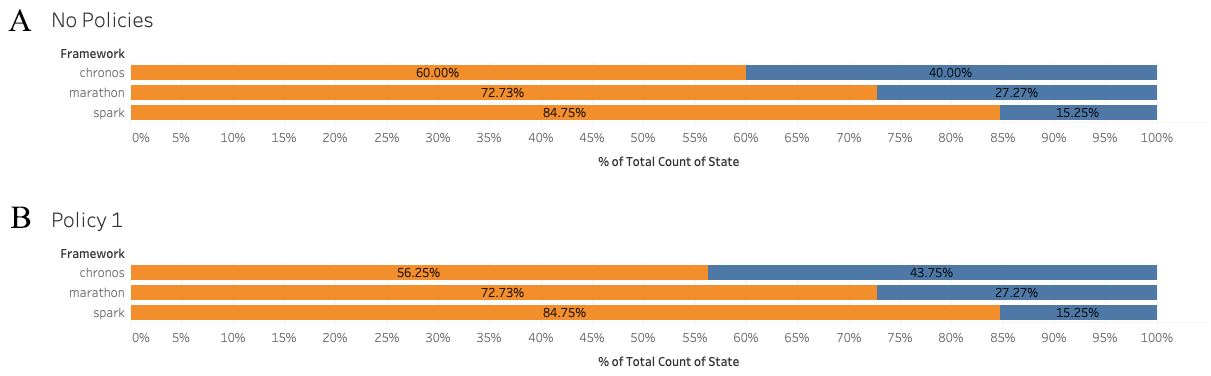
\includegraphics[width=14cm]{./image/chap4/finfail0-1.png}}
    \caption{Number of finished and failed tasks before and after using FDP}\label{fig:finfail0-1}
    (A) is before using FDP and (B) is  after using FDP
\end{figure}
\begin{figure}[!h]\centering
    \setlength{\fboxrule}{0mm} % can define this in the preamble
    \setlength{\fboxsep}{0cm}
    \fbox{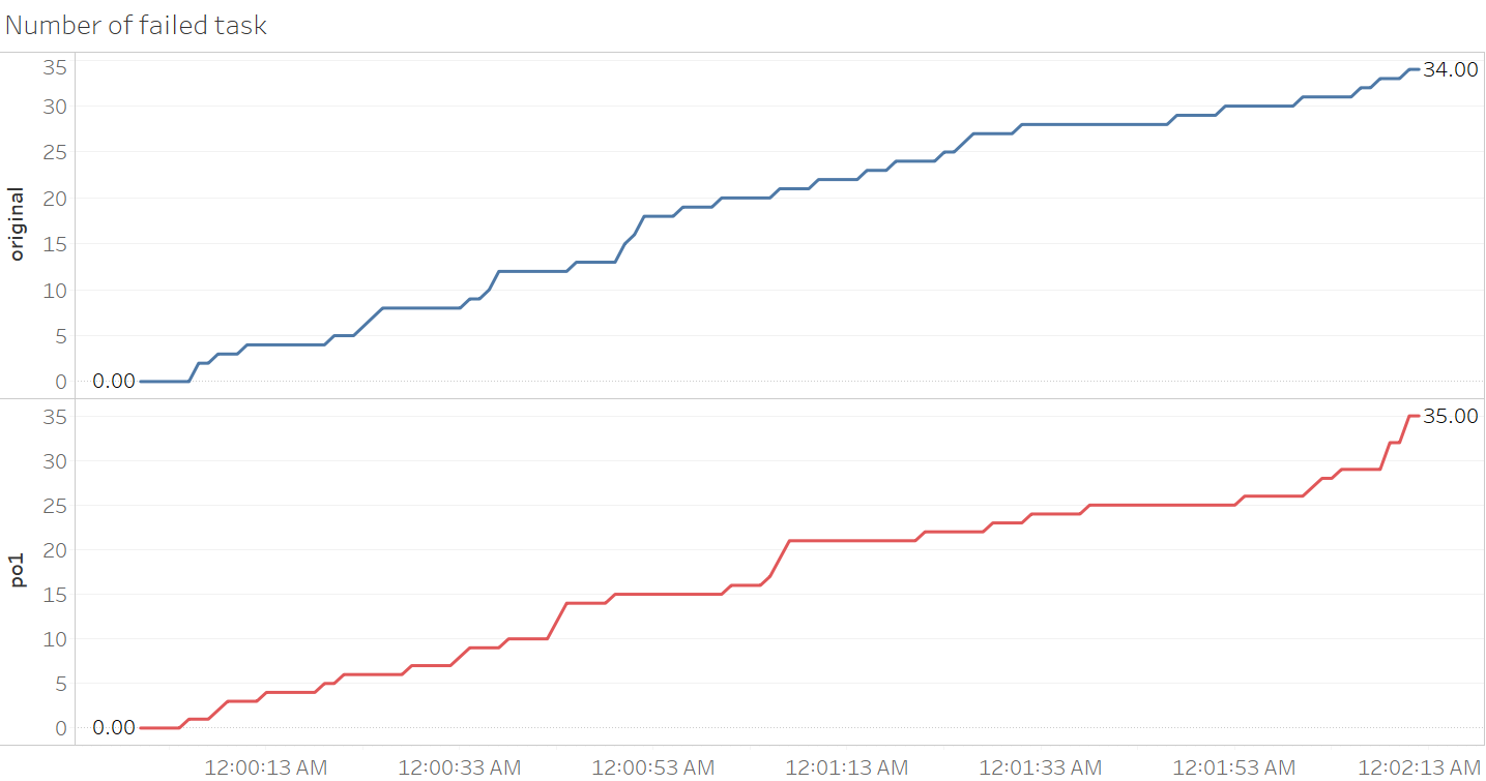
\includegraphics[width=14cm]{./image/chap4/po1-fail.png}}
    \caption{Growth rate of fail task before and after using FDP}\label{fig:fail1}
\end{figure}

% po1 CPU and mem
\newpage
  \item \textbf{CPU and memory utilization}
  \newline
  The averages of CPU and memory utilization of cluster framework before and after used this policy is shown in \textbf{Table}~\ref{tbl:po1CPUMem}. From the table, both CPU and memory utilization average were increased after used this policy. The amounts of CPU and memory utilization before and after used this policy in each time is shown in \textbf{Figure}~\ref{fig:cpu1} and \textbf{Figure}~\ref{fig:mem1}. 
  \begin{table}[!h]
  \caption{Average of CPU and memory utilization before and after using FDP.}\label{tbl:po1CPUMem}
  \begin{tabular}{@{}|p{0.2\textwidth}|p{0.35\textwidth}|p{0.35\textwidth}|}
   \hline
   \textbf{} & \textbf{Before} & \textbf{After} \\ 
   \hline
   \textbf{CPU} & 80.23\% & 80.53\% \\ 
   \hline
   \textbf{Memory} & 39.46\% & 44.40\% \\ 
   \hline                     
  \end{tabular}
\end{table}
\begin{figure}[!h]\centering
    \setlength{\fboxrule}{0mm} % can define this in the preamble
    \setlength{\fboxsep}{0cm}
    \fbox{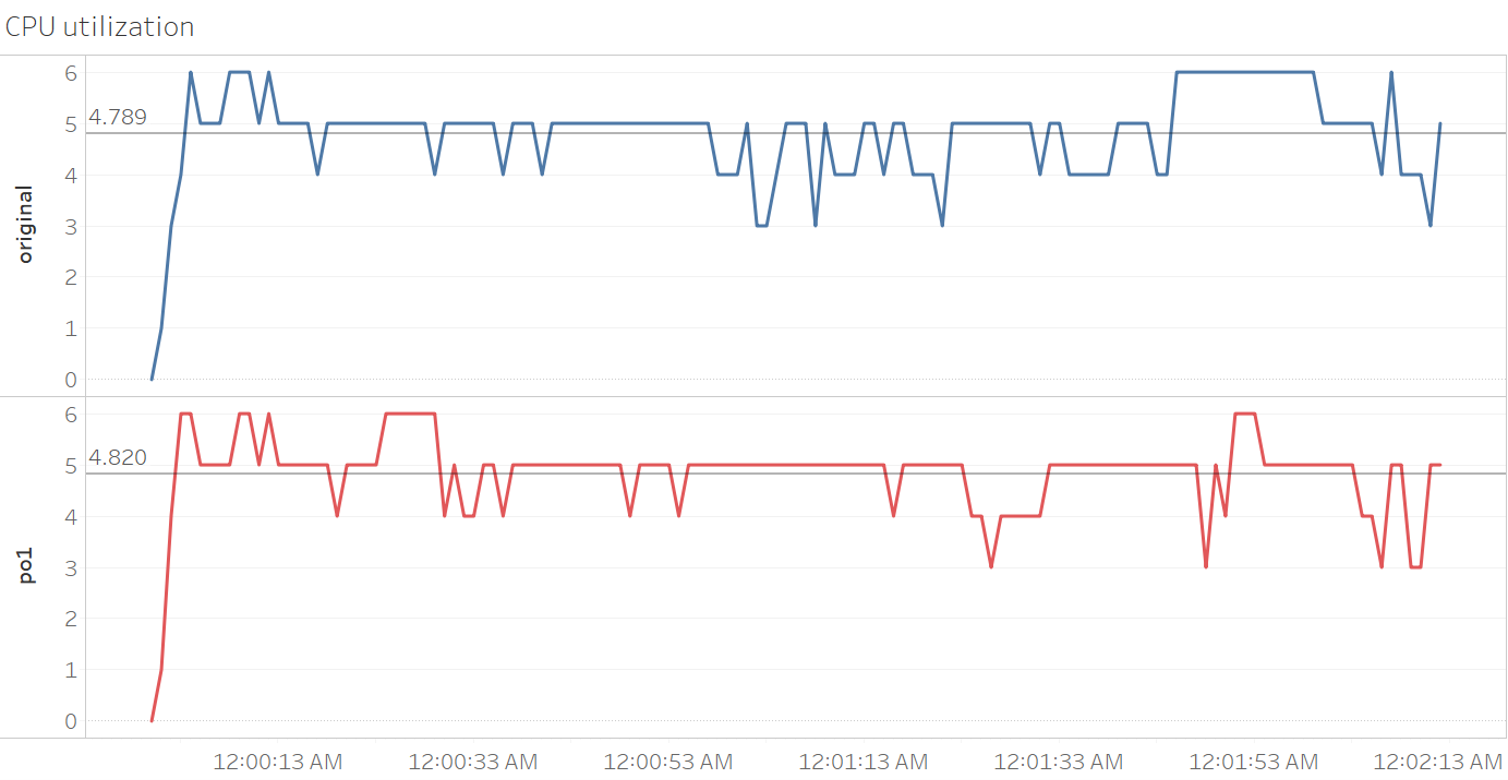
\includegraphics[width=14cm]{./image/chap4/po1-cpu.png}}
    \caption{CPU utilization before and after using FDP}\label{fig:cpu1}
\end{figure}
\begin{figure}[!h]\centering
    \setlength{\fboxrule}{0mm} % can define this in the preamble
    \setlength{\fboxsep}{0cm}
    \fbox{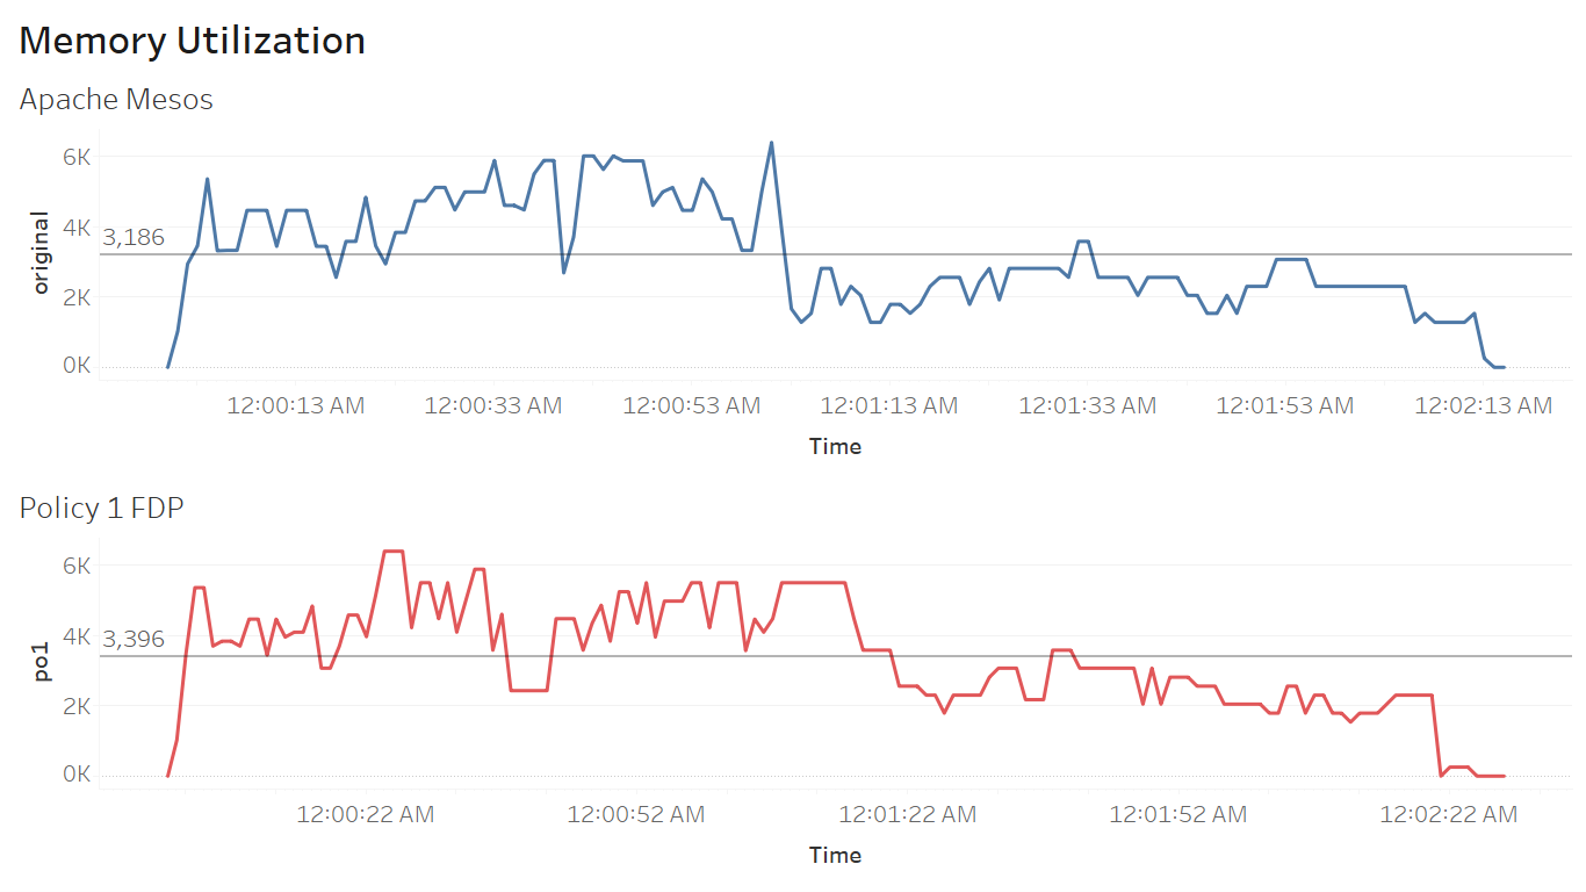
\includegraphics[width=14cm]{./image/chap4/po1-mem.png}}
    \caption{Memory utilization before and after using FDP}\label{fig:mem1}
\end{figure}

%%% po1 load
  \item \textbf{System load}
  \newline
  The result of system load in this cluster before and after used this policy is shown in \textbf{Figure}~\ref{fig:load1}. System load average before using FDP is 2.085 and after is 3.033. So, system is busier when applied this policy.
\begin{figure}[!h]\centering
    \setlength{\fboxrule}{0mm} % can define this in the preamble
    \setlength{\fboxsep}{0cm}
    \fbox{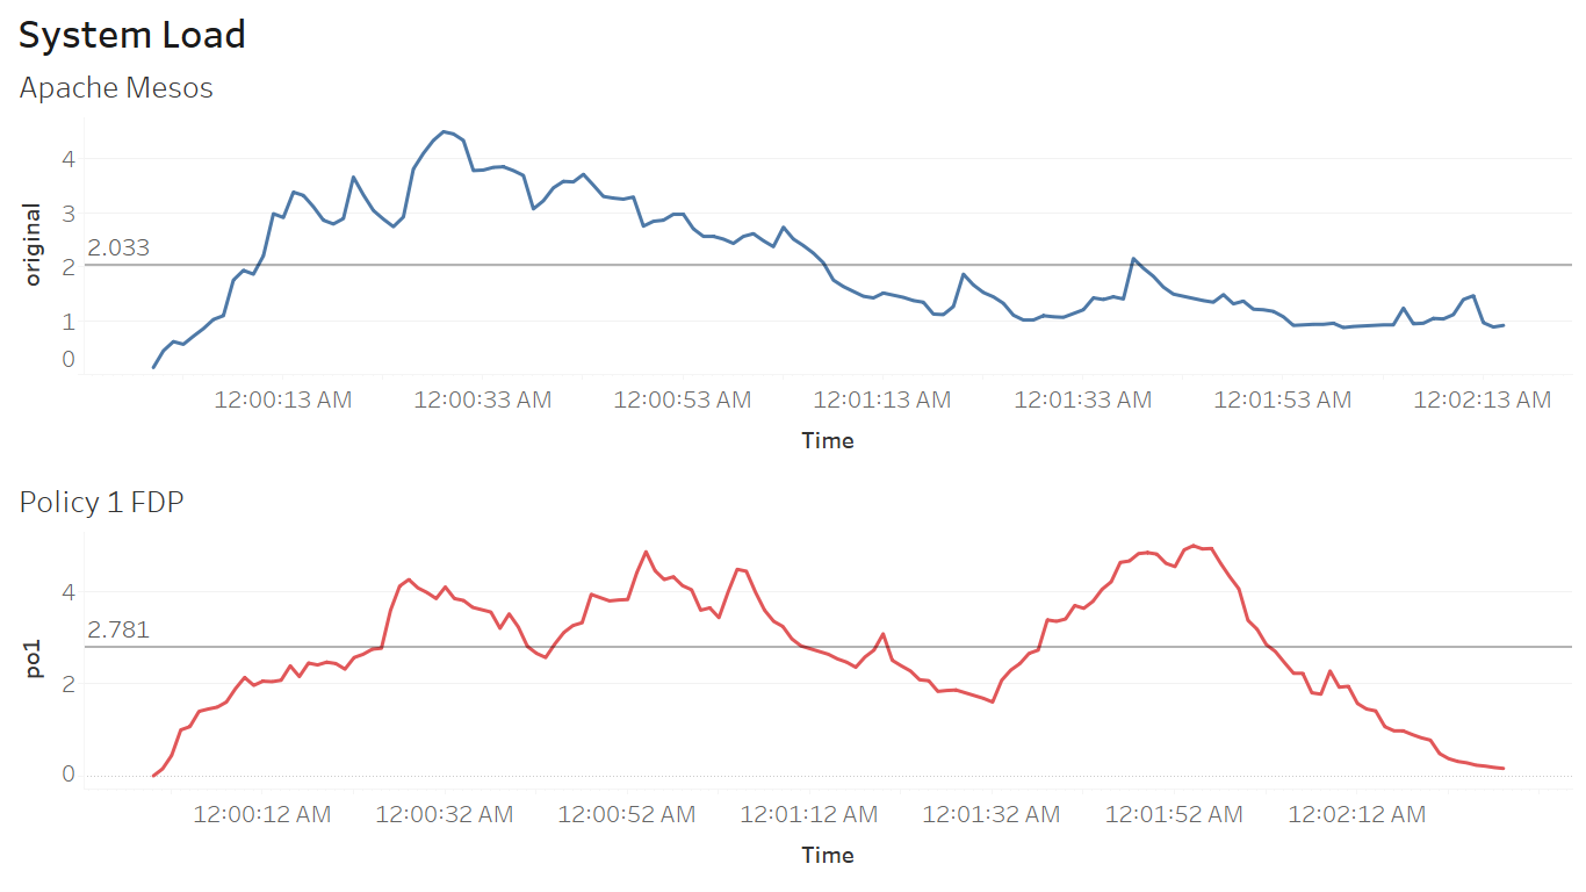
\includegraphics[width=14cm]{./image/chap4/po1-load.png}}
    \caption{System load before and after using FDP}\label{fig:load1}
\end{figure}
\end{enumerate}
%%% po1 conclusion
\textbf{Conclusion of First Demand Share Policy (FDP)}
\newline
\hspace{10mm}First Demand Policy can improve fairness of running tasks in a period of time. The number of failed tasks is still the same in the most of frameworks. Only Chronos failed task is decrease by 3.75\%. Also, failure rate of failed tasks, resource utilization and system load are not improved. 


%%%%%%%%%% Policy 2: Success Rate Prediction %%%%%%%%%%%%
\section{Policy 2: Success Rate Prediction}  
\hspace{10mm}The result of submitted task is shown in \textbf{Figure}~\ref{fig:task2}.

\begin{figure}[!h]\centering
    \setlength{\fboxrule}{0mm} % can define this in the preamble
    \setlength{\fboxsep}{0cm}
    \fbox{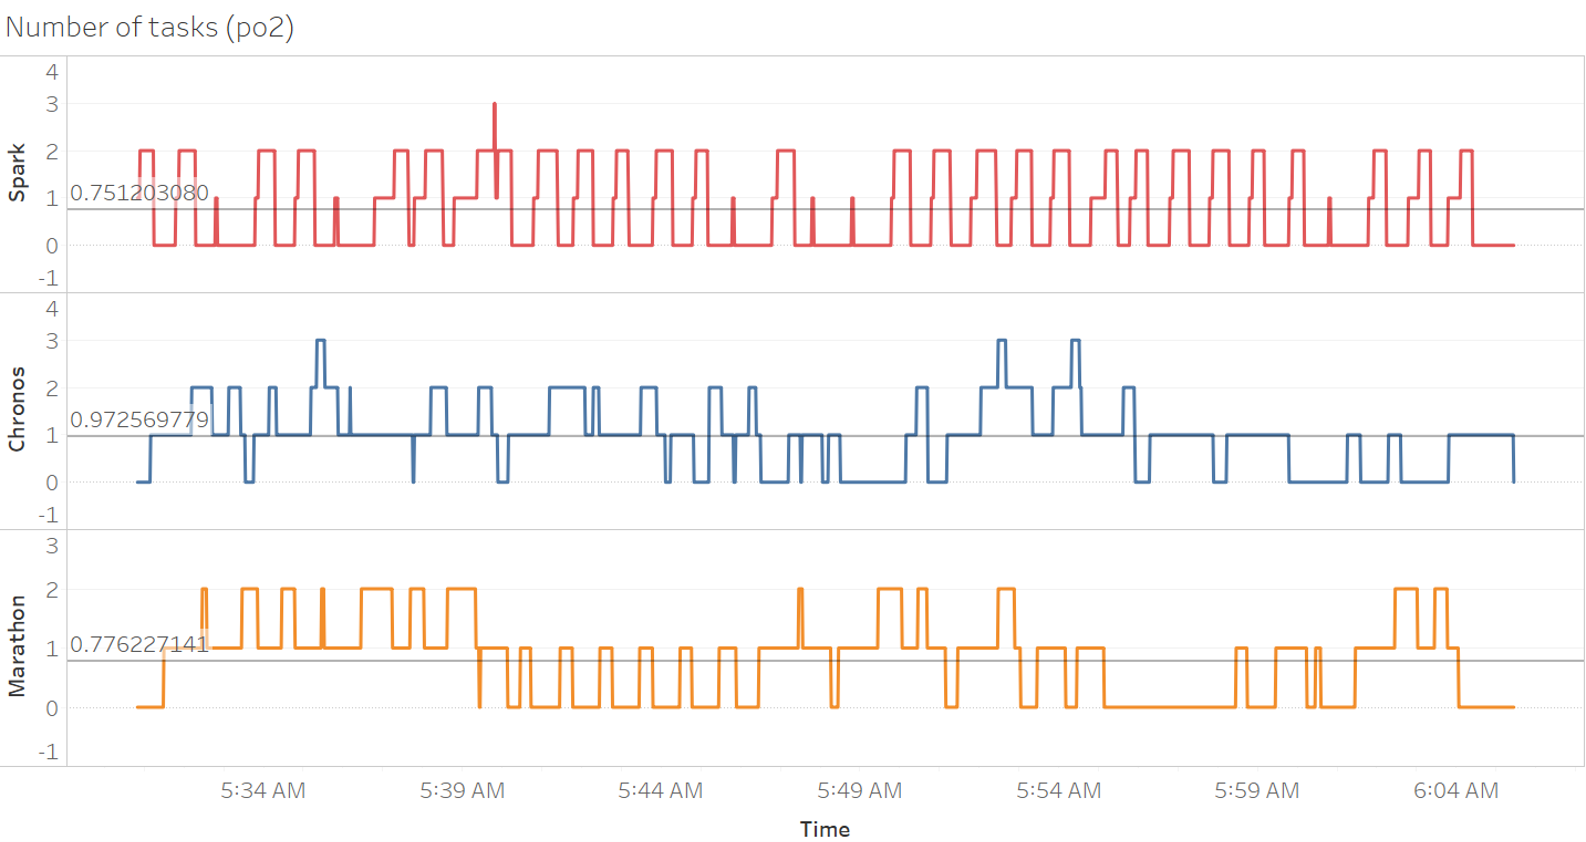
\includegraphics[width=14cm]{./image/chap4/task2.png}}
    \caption{Number of tasks for each framework after using Success Rate Prediction}\label{fig:task2}
\end{figure}

\hspace{10mm}There is a little improvement in fairness as shown in \textbf{Figure}~\ref{fig:task2}. Each framework had almost the same approximate number of tasks, which is 0.97. After calculating different average, the values are (0.7512, 0.9725, and 0.7762), the result is 0.147. So, this policy can improve fairness compared to the default policy 0.3736. Then it comes to the result of fairness improvement by 60\% and the fairness increased by 42.8\%
\newline
This project also considered these other matrices after applying this policy:  
\begin{enumerate}
%%% po2 fail task
  \item \textbf{Failed task}
  \newline
  The result of failed and finished tasks for each framework before and after applied this policy is shown in \textbf{Figure}~\ref{fig:finfail0-2}.The orange color shows percent of finished tasks and the blue one shows percent of failed tasks. The number of failed tasks in every framework was decreased. In \textbf{Figure}~\ref{fig:fail2} shows that growth rate of failed tasks is downward when used this policy. The slope was decreased from 0.258 to 0.152. So, this policy can reduce the number of failed tasks in every framework and decrease its failure rate.
  \begin{figure}[!h]\centering
    \setlength{\fboxrule}{0mm} % can define this in the preamble
    \setlength{\fboxsep}{0cm}
    \fbox{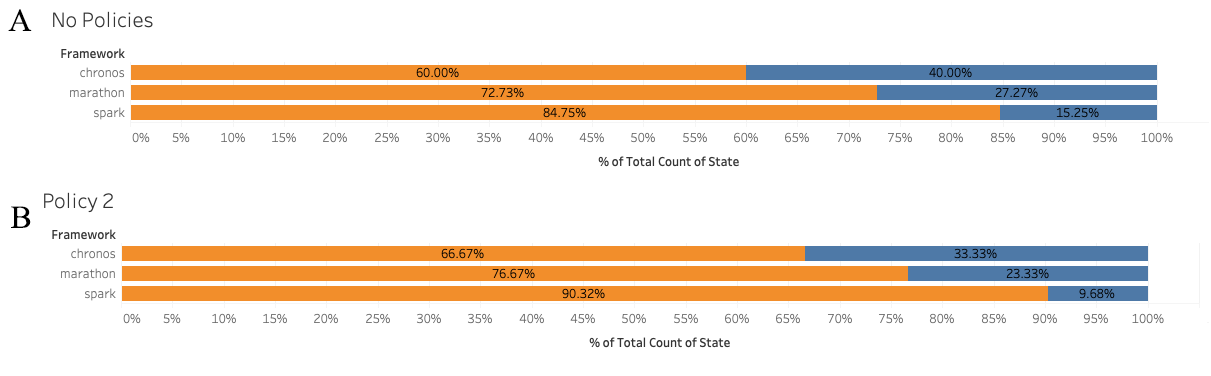
\includegraphics[width=14cm]{./image/chap4/finfail0-2.png}}
    \caption{Number of finished and failed tasks before and after using Success Rate Prediction}\label{fig:finfail0-2}
    (A) is before using Success Rate Prediction and (B) is  after using Success Rate Prediction
\end{figure}
\begin{figure}[!h]\centering
    \setlength{\fboxrule}{0mm} % can define this in the preamble
    \setlength{\fboxsep}{0cm}
    \fbox{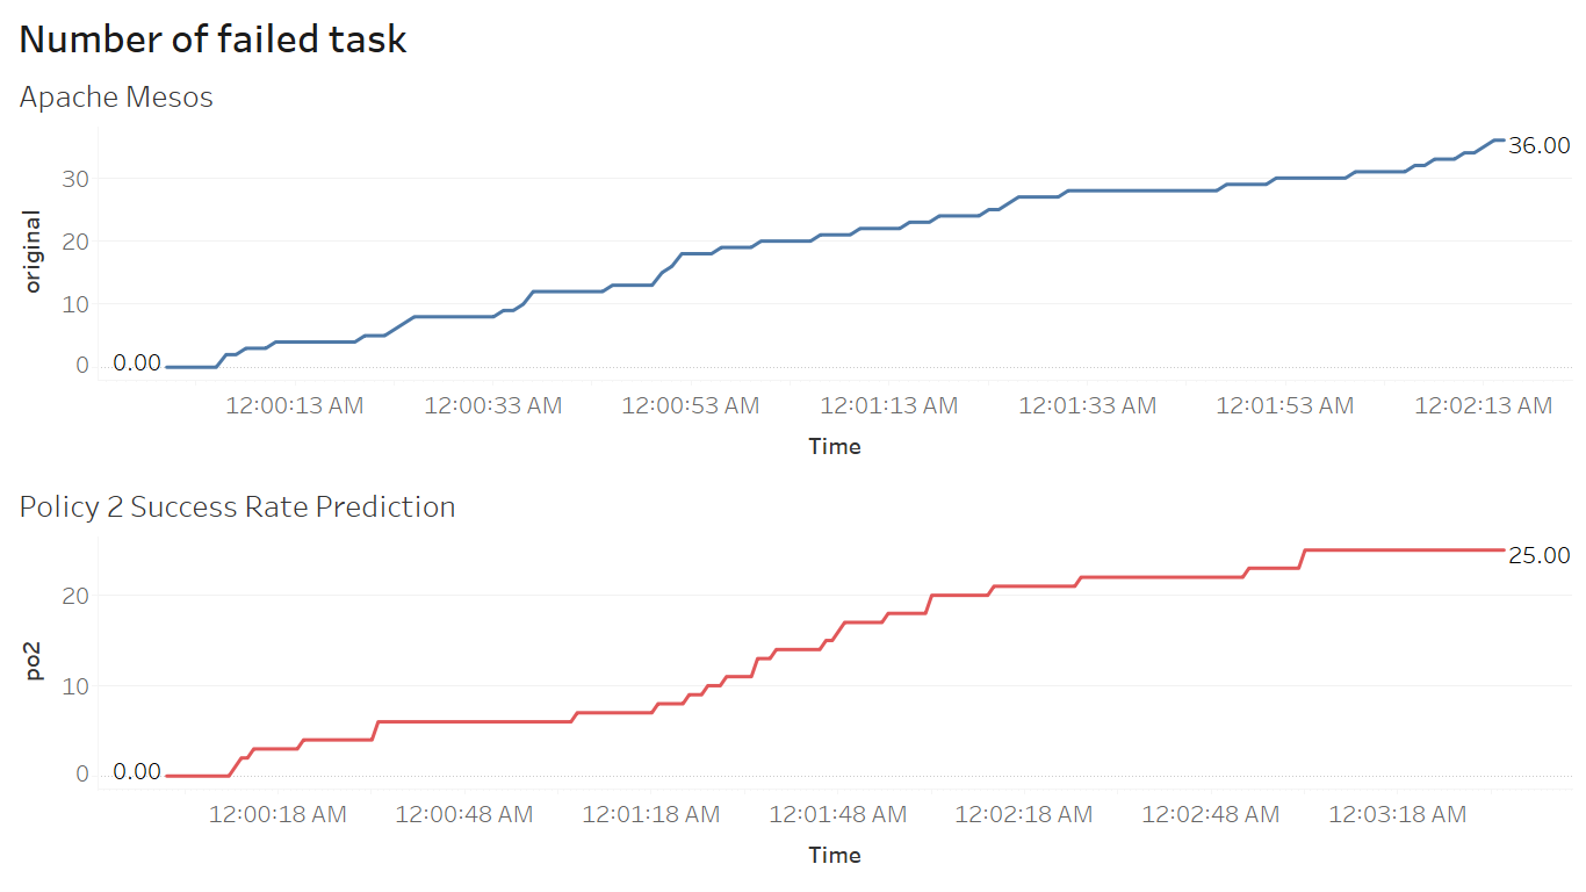
\includegraphics[width=14cm]{./image/chap4/po2-fail.png}}
    \caption{Growth rate of fail task before and after using Success Rate Prediction}\label{fig:fail2}
\end{figure}

%%% po2 CPU and mem
\newpage
  \item \textbf{CPU and memory utilization}
  \newline
  The averages of CPU and memory utilization of cluster framework before and after used this policy is shown in \textbf{Table}~\ref{tbl:po2CPUMem}. From the table, both CPU and memory utilization average were decreased after used this policy. The amounts of CPU and memory utilization before and after used this policy in each time is shown in \textbf{Figure}~\ref{fig:cpu2} and \textbf{Figure}~\ref{fig:mem2}. 
  \begin{table}[!h]
  \caption{Average of CPU and memory utilization before and after using FDP.}\label{tbl:po2CPUMem}
  \begin{tabular}{@{}|p{0.2\textwidth}|p{0.35\textwidth}|p{0.35\textwidth}|}
   \hline
   \textbf{} & \textbf{Before} & \textbf{After} \\ 
   \hline
   \textbf{CPU} & 80.23\% & 43.73\% \\ 
   \hline
   \textbf{Memory} & 39.46\% & 22.04\% \\ 
   \hline                     
  \end{tabular}
\end{table}
\begin{figure}[!h]\centering
    \setlength{\fboxrule}{0mm} % can define this in the preamble
    \setlength{\fboxsep}{0cm}
    \fbox{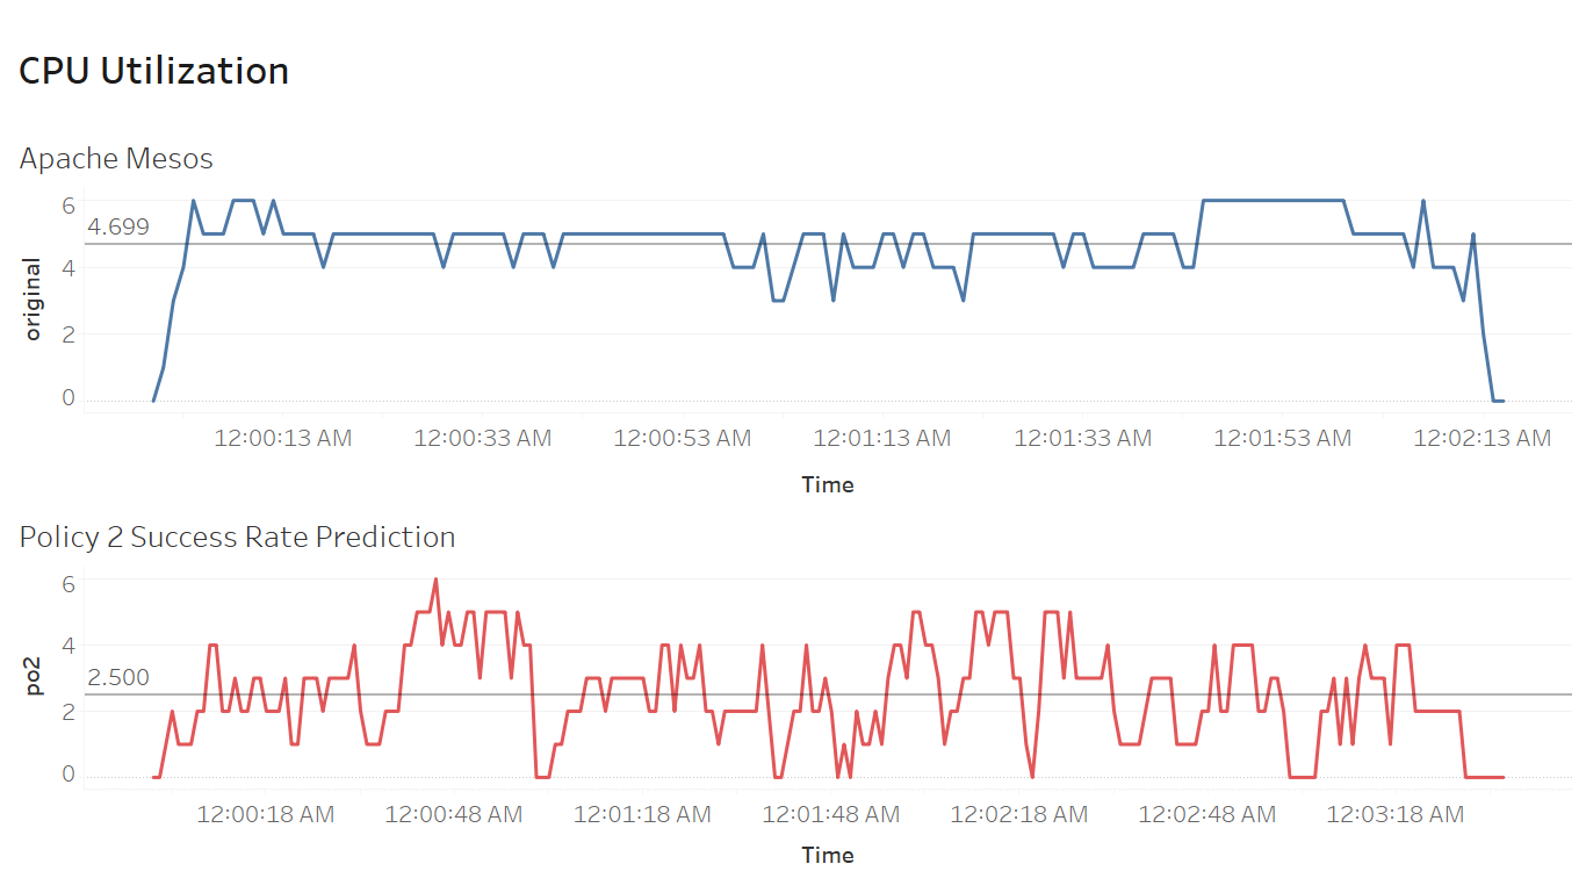
\includegraphics[width=14cm]{./image/chap4/po2-cpu.png}}
    \caption{CPU utilization before and after using Success Rate Prediction}\label{fig:cpu2}
\end{figure}
\begin{figure}[!h]\centering
    \setlength{\fboxrule}{0mm} % can define this in the preamble
    \setlength{\fboxsep}{0cm}
    \fbox{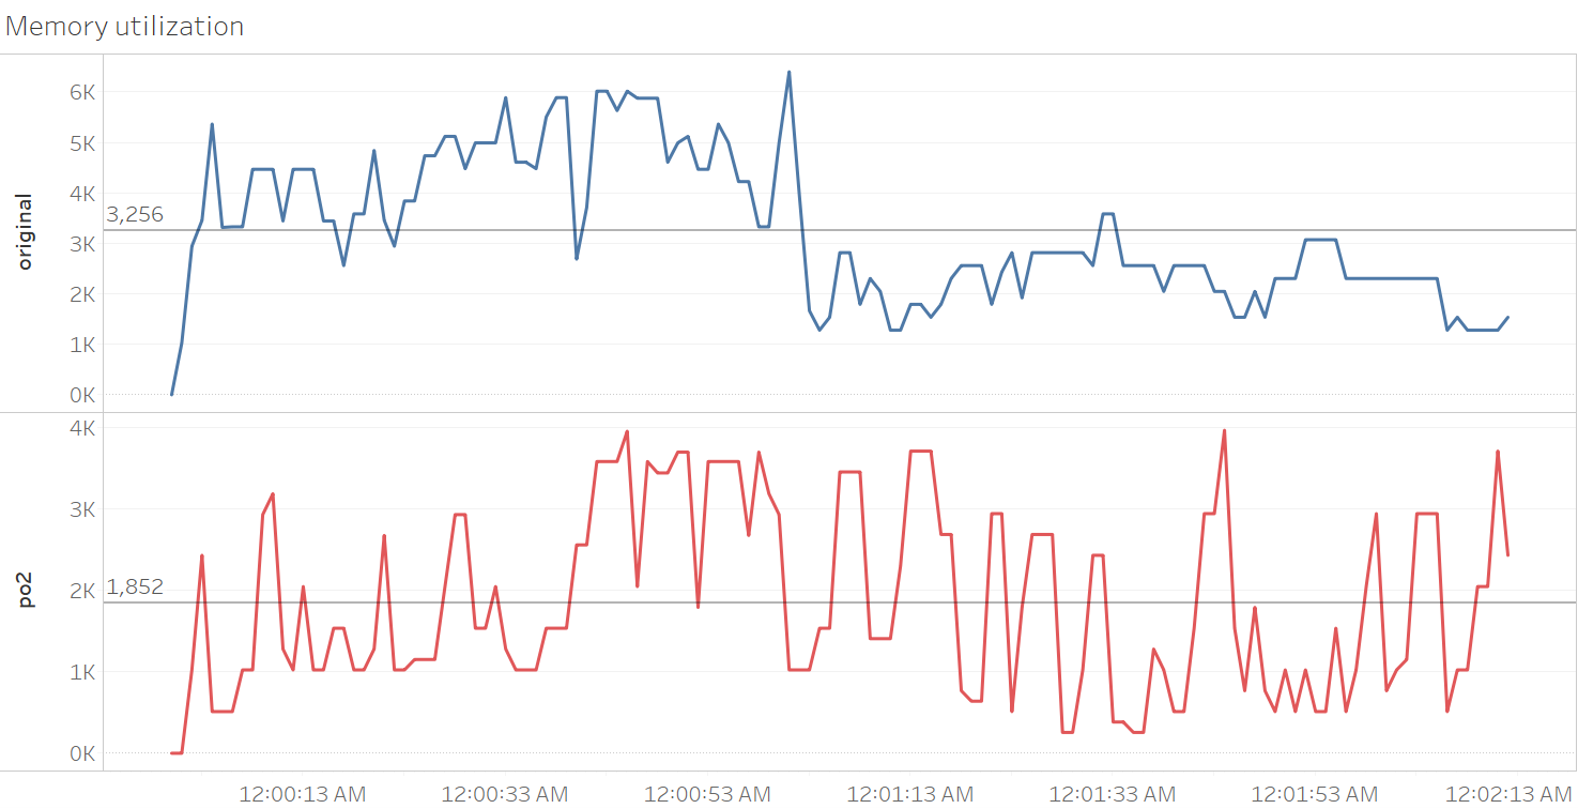
\includegraphics[width=14cm]{./image/chap4/po2-mem.png}}
    \caption{Memory utilization before and after using Success Rate Prediction}\label{fig:mem2}
\end{figure}

%%% po2 load
  \item \textbf{System load}
  \newline
  The result of system load in this cluster before and after used this policy is shown in \textbf{Figure}~\ref{fig:load2}. System load average before using FDP is 2.058 and after is 1.188. So, system is less busy when applied this policy.
\begin{figure}[!h]\centering
    \setlength{\fboxrule}{0mm} % can define this in the preamble
    \setlength{\fboxsep}{0cm}
    \fbox{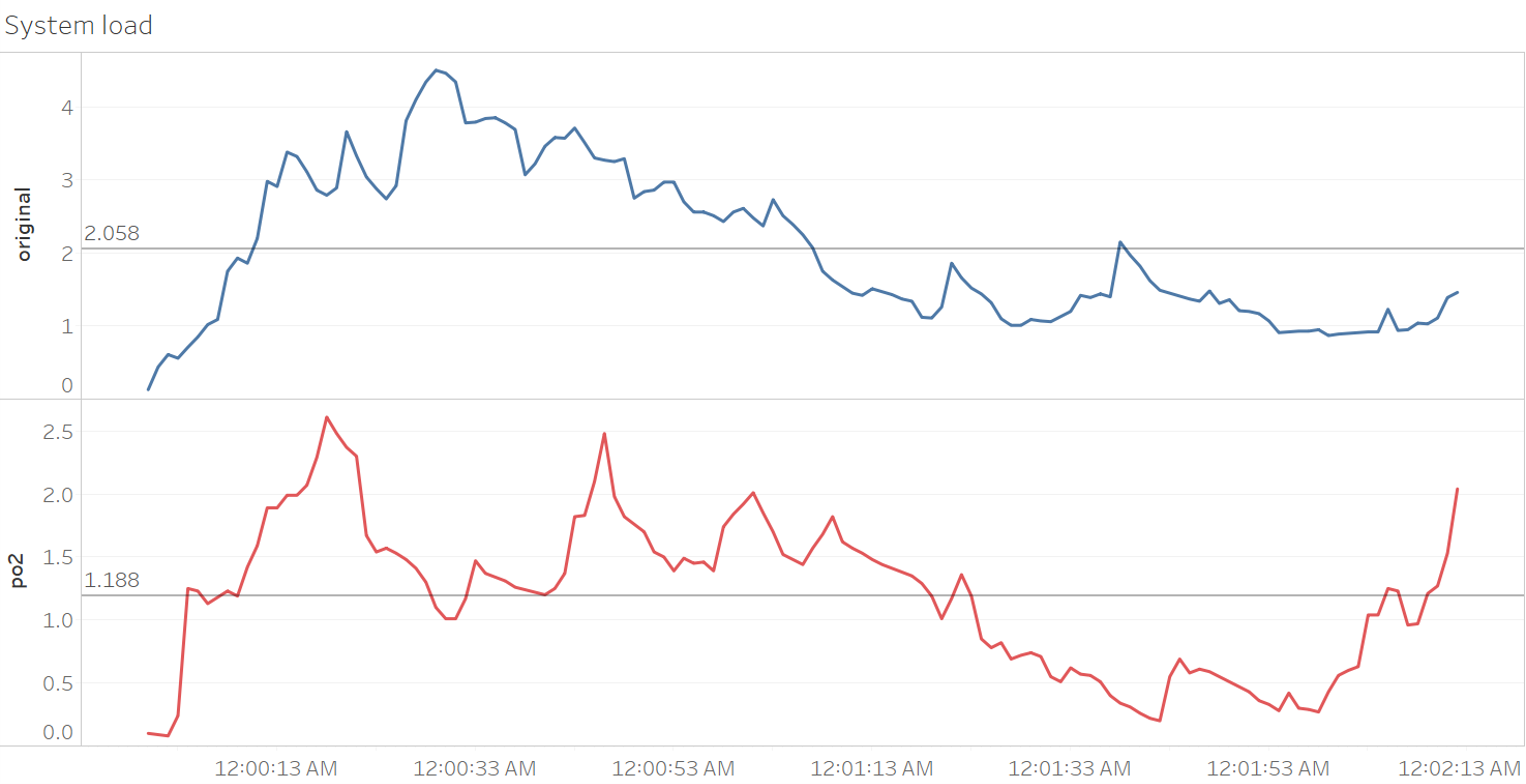
\includegraphics[width=14cm]{./image/chap4/po2-load.png}}
    \caption{System load before and after using Success Rate Prediction}\label{fig:load2}
\end{figure}
\end{enumerate}
%%% po2 conclusion
\textbf{Conclusion of Success Rate Prediction}
\newline
\hspace{10mm}Success Rate Prediction can improve fairness of running tasks by only 60\%. The number of failed tasks is reduced by 7.3\%. Also, failure rate of failed tasks, resource utilization, and system load are improved.

%%%%%%%%%% Policy 3: Hybrid Policy %%%%%%%%%%%%
\section{Policy 3: Hybrid Policy}  
\hspace{10mm}Hybrid Policy is combined FDP and Success Rate Prediction. The result of submitted task is shown in \textbf{Figure}~\ref{fig:task3}.

\begin{figure}[!h]\centering
    \setlength{\fboxrule}{0mm} % can define this in the preamble
    \setlength{\fboxsep}{0cm}
    \fbox{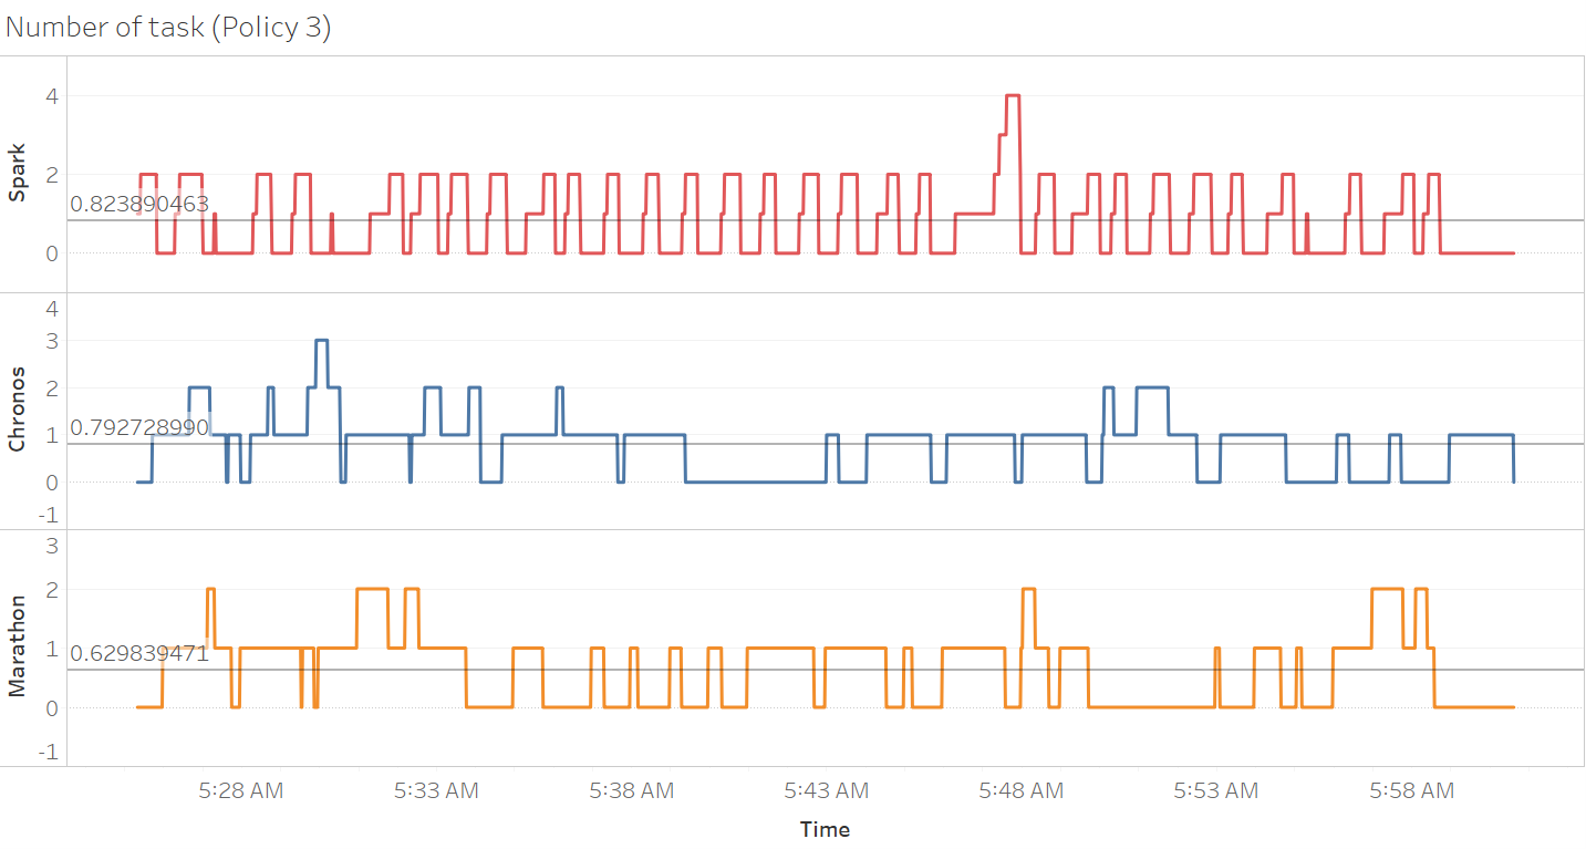
\includegraphics[width=14cm]{./image/chap4/task3.png}}
    \caption{Number of tasks for each framework after using Hybrid Policy}\label{fig:task3}
\end{figure}

\hspace{10mm}In \textbf{Figure}~\ref{fig:task3}, There is a little improvement in fairness as shown. Each framework had almost the same approximate number of tasks, which is 0.74. After calculated different average, the values are (0.823, 0.7927, and 0.6298), the result is 0.1293. So, this policy can improve fairness compared to the default policy 0.3736. Then it comes to the result of fairness improvement by 65.40\%, compared to the first policy, the fairness improved by 49.68\% and compared to the second policy, the fairness improved by 12\%
\newline
This project also considered these other matrices after applying this policy: 
\begin{enumerate}
%%% po3 fail task
  \item \textbf{Failed task}
  \newline
  The result of failed and finished tasks for each framework before and after applied both policies is shown in  \textbf{Figure}~\ref{fig:finfail0-3}. The orange color shows percent of finished tasks and the blue one shows percent of failed tasks. The number of failed tasks in every framework was decreased by this policy. In \textbf{Figure}~\ref{fig:fail3} shows that growth rate of failed tasks is upward when used this policy. The slope decreased from 0.258 to 0.06. So, this policy cannot reduce the number of failed tasks in every framework and its failure rate.
  \begin{figure}[!h]\centering
    \setlength{\fboxrule}{0mm} % can define this in the preamble
    \setlength{\fboxsep}{0cm}
    \fbox{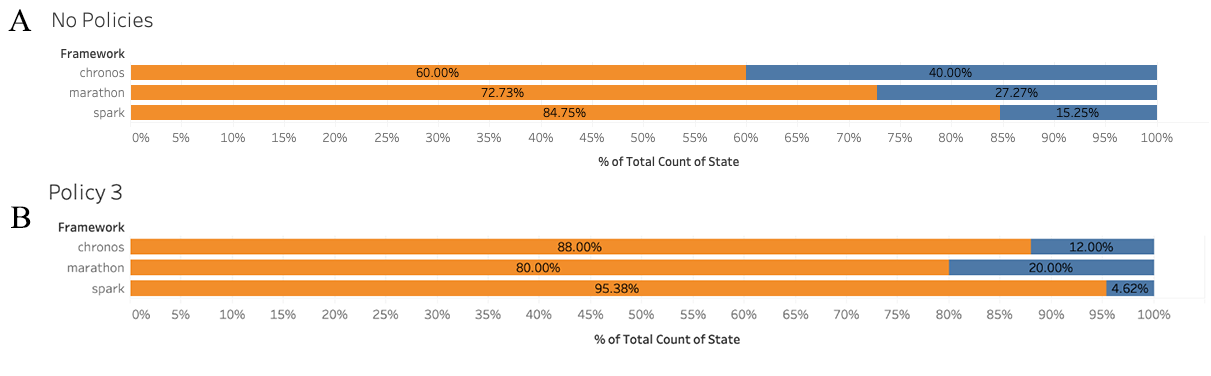
\includegraphics[width=14cm]{./image/chap4/finfail0-3.png}}
    \caption{Number of finished and failed tasks before and after using Hybrid Policy}\label{fig:finfail0-3}
    (A) is before using Hybrid Policy and (B) is  after using Hybrid Policy
\end{figure}
\begin{figure}[!h]\centering
    \setlength{\fboxrule}{0mm} % can define this in the preamble
    \setlength{\fboxsep}{0cm}
    \fbox{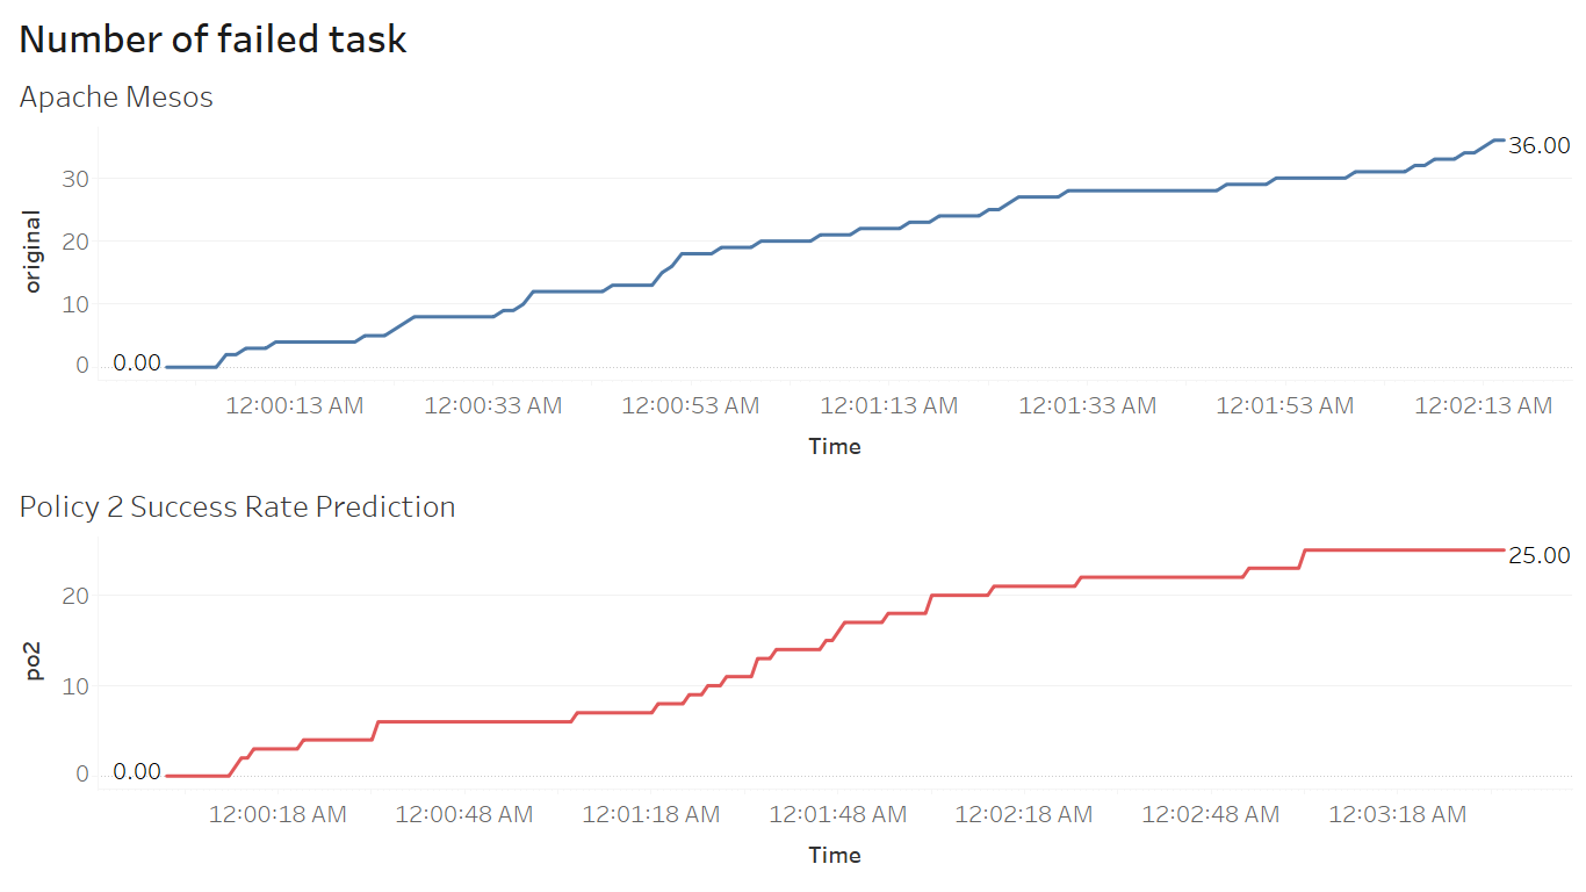
\includegraphics[width=14cm]{./image/chap4/po2-fail.png}}
    \caption{Growth rate of fail task before and after using Hybrid Policy}\label{fig:fail3}
\end{figure}

%%%po3 CPU and mem
  \item \textbf{CPU and memory utilization}
  \newline
The averages of CPU and memory utilization of cluster framework before and after used this policy is shown in \textbf{Table}~\ref{tbl:po3CPUMem}. From the table, both CPU and memory utilization average were decreased after used this policy. The amounts of CPU and memory utilization before and after used this policy in each time is shown in Figure \textbf{Figure}~\ref{fig:cpu3} and\textbf{Figure}~\ref{fig:mem3}.    
  \begin{table}[!h]
  \caption{Average of CPU and memory utilization before and after using both FDP and success rate prediction.}\label{tbl:po3CPUMem}
  \begin{tabular}{@{}|p{0.2\textwidth}|p{0.35\textwidth}|p{0.35\textwidth}|}
   \hline
   \textbf{} & \textbf{Before} & \textbf{After} \\ 
   \hline
   \textbf{CPU} & 80.23\% & 45.73\% \\ 
   \hline
   \textbf{Memory} & 39.46\% & 26.33\% \\ 
   \hline                     
  \end{tabular}
\end{table}
\begin{figure}[!h]\centering
    \setlength{\fboxrule}{0mm} % can define this in the preamble
    \setlength{\fboxsep}{0cm}
    \fbox{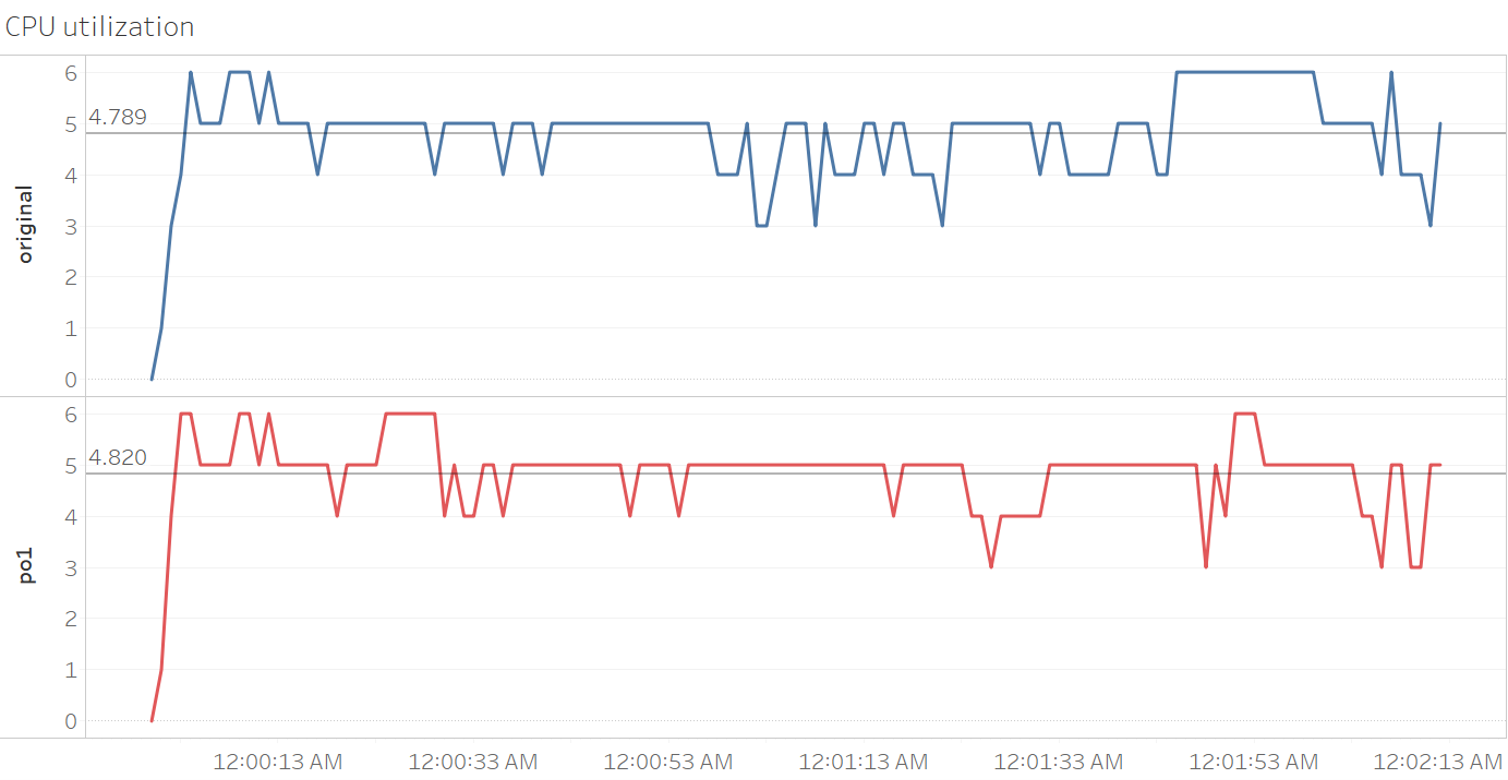
\includegraphics[width=14cm]{./image/chap4/po1-cpu.png}}
    \caption{CPU utilization before and after using Hybrid Policy}\label{fig:cpu3}
\end{figure}
\begin{figure}[!h]\centering
    \setlength{\fboxrule}{0mm} % can define this in the preamble
    \setlength{\fboxsep}{0cm}
    \fbox{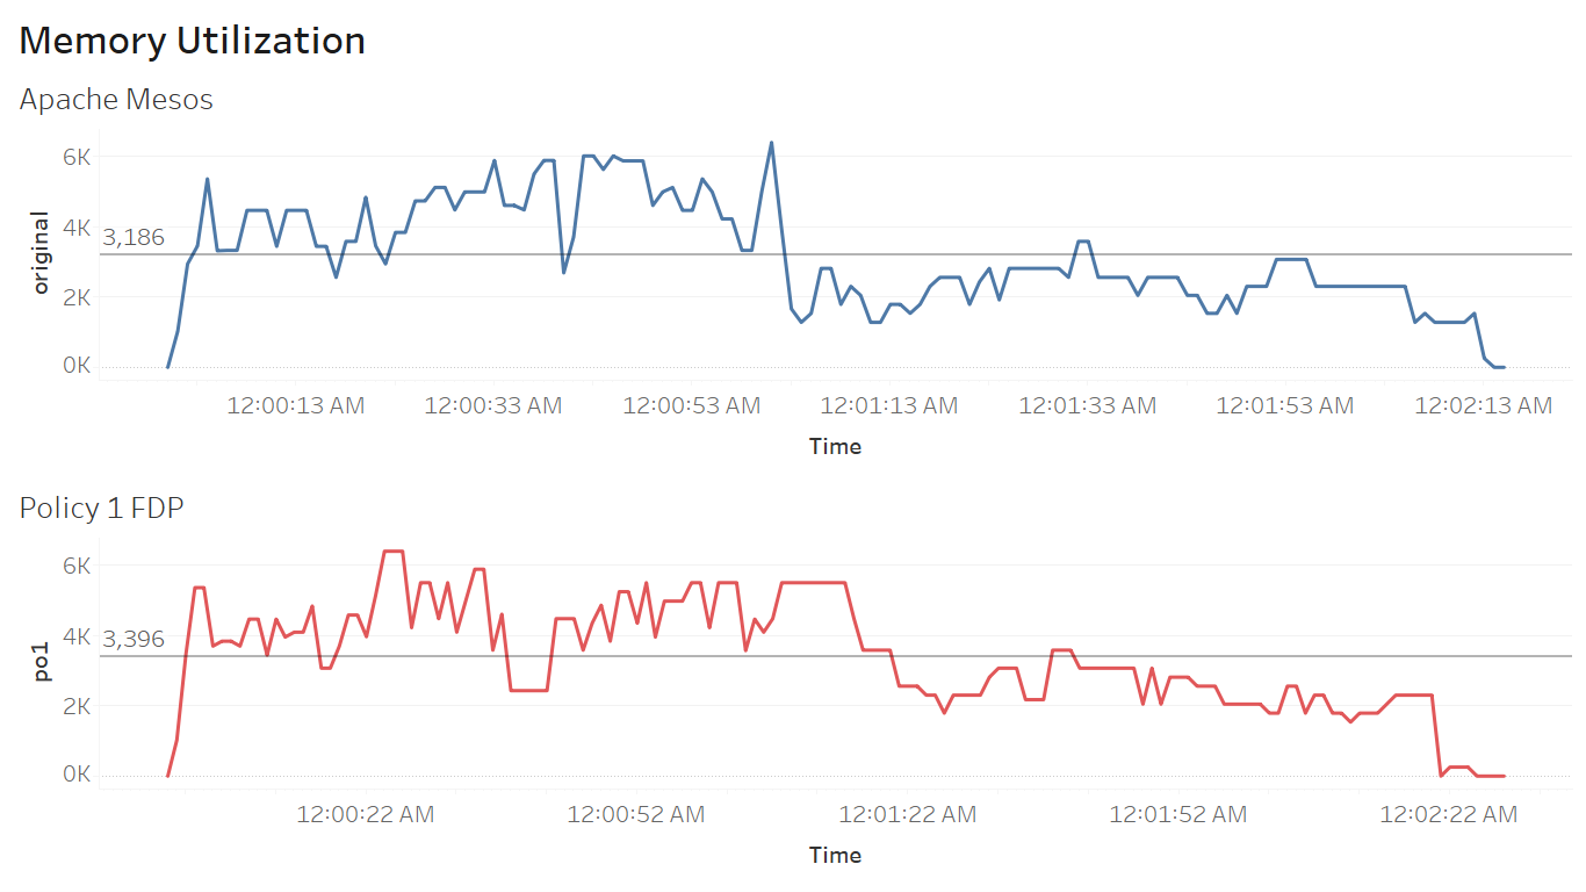
\includegraphics[width=14cm]{./image/chap4/po1-mem.png}}
    \caption{Memory utilization before and after using Hybrid Policy}\label{fig:mem3}
\end{figure}

%%%po3 load
  \item \textbf{System load}
  \newline
  The result of system load in this cluster before and after used this policy is shown in \textbf{Figure}~\ref{fig:load3}. System load average before using FDP is 2.058 and after is 0.579. So, system is less busy when applied this policy.
\begin{figure}[!h]\centering
    \setlength{\fboxrule}{0mm} % can define this in the preamble
    \setlength{\fboxsep}{0cm}
    \fbox{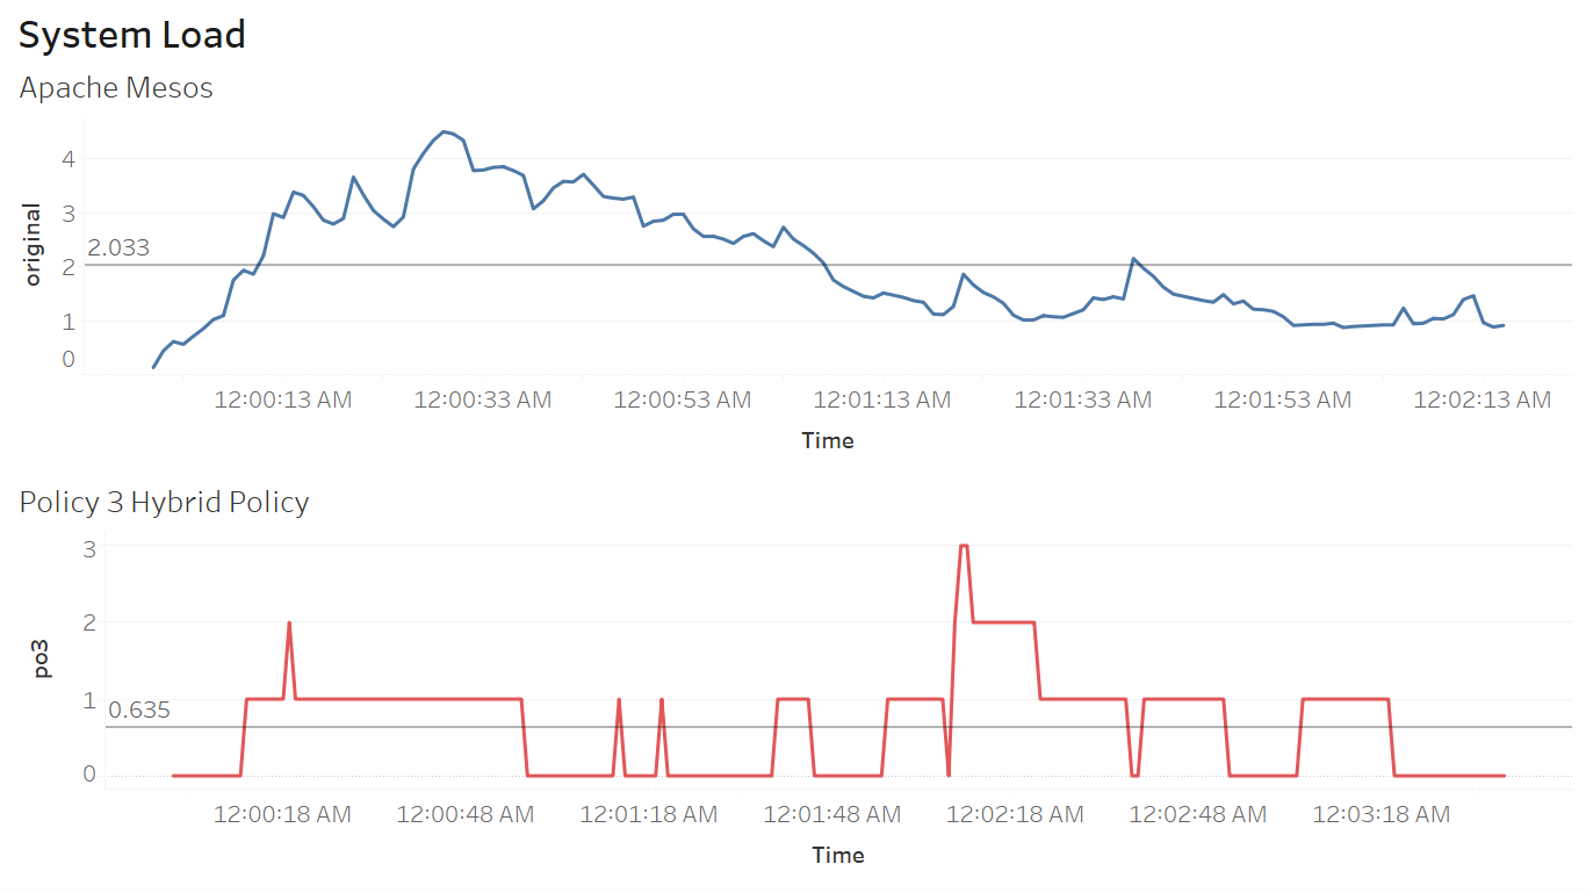
\includegraphics[width=14cm]{./image/chap4/po3-load.png}}
    \caption{System load before and after using Success Rate Prediction}\label{fig:load3}
\end{figure}
\end{enumerate}

%%% po3 conclusion
\textbf{Conclusion of Hybrid Policy}
\newline
\hspace{10mm}Hybrid Policy can achieve the best results in terms of failure task and other metrics. Fairness of running tasks is improve by only 65.4\%. The number of failed tasks is reduced by 15.3\%. Also, failure rate of failed tasks, resource utilization and system load are improved.

%%%%%%%%%% Summary of Result %%%%%%%%%%%%
\section{Summary of Result}  
\hspace{10mm}The \textbf{Table}~\ref{tbl:chap4Sum} is shown result of all metrics from original Apache Mesos, Apache Mesos applied with First demand policy, Apache Mesos applied with Success Rate Prediction and apache Mesos applied with Hybrid Policy.
  \begin{table}[!h]
  \caption{Failure task and other metrics.}\label{tbl:chap4Sum}
  \begin{tabular}{@{}|p{0.2\textwidth}|p{0.1\textwidth}|p{0.1\textwidth}|p{0.1\textwidth}|p{0.1\textwidth}|p{0.1\textwidth}|p{0.1\textwidth}|}
   \hline
   \textbf{Policy} & \textbf{Fairness} & \textbf{Number of failed tasks (tasks)} & \textbf{Average of CPU utilization} & \textbf{Average of Memory utilization} & \textbf{Average of System load (tasks)} & \textbf{Running Time(min)} \\
   \hline
   \textbf{Original Apache Mesos}& 0.3736 & 34& 80.23\% & 39.46\% &2.083& 24.26 \\
   \hline
   \textbf{First demand policy} & 0.257& 35& 80.75\% & 40.40\% & 3.067& 24.26\\
   \hline
   \textbf{Success Rate Prediction}& 0.147& 20& 43.73\% & 22.04\%& 1.188& 34.37 \\
   \hline
   \textbf{Hybrid Policy} & 0.1293 & 8 & 45.73\% & 26.33\% & 0.579  & 35.17 \\ 
   \hline                   
  \end{tabular}
\end{table}


%%%%%%%%%%%%%%%%%%%%%%%%%%%%%%%%%%%%%%%%%%%%%%%%%%%%%%%%%%%%%%%
%%%%%%%%%%%%%%%%%%%% Conclusions %%%%%%%%%%%%%%%%%%%%%%%%%%%%%
%%%%%%%%%%%%%%%%%%%%%%%%%%%%%%%%%%%%%%%%%%%%%%%%%%%%%%%%%%%%%%%
\chapter{Conclusions}

\hspace{10mm}In this chapter, there are conclusion of this project, its result, discussion about the result and future work that could be done to improve this project.

%%%%%%%%%% Result and Discussion %%%%%%%%%%%%
\section{Result and Discussion}
\hspace{10mm}As previous mentioned, this project has three policies attached to NKR-scheduler. The tasks were submitted to NKR-scheduler. After \textbf{First Demand Policy} is applied, the fairness in system is decreased by 16.6\% and the other metrics such as CPU utilization, memory utilization, failure rate, etc., were increased. The result did not improve performance as expected, and it was found that fairness has a correlation with failure task. Next experiment applies \textbf{Success Rate Prediction}. The failure rate was improved by nearly 7.3\% and the others metrics were significantly improved. However, the failure rate did not meet the criteria as expected, and fairness did not improve. Therefore, the last policy called Hybrid Policy was developed. The result shown that the failure rate was improved by 15.3\% and the other metric were improved. After simulated task were scheduling, we found Spark was configured with a relatively greedier scheduling policy compared to the other frameworks. This type of scheduling can significantly affect the other frameworks to manage resources utilization. As a result, spark can run more tasks at the beginning and come with the highest number of success tasks compared to other frameworks, whereas other frameworks required much more time to complete and caused higher failure rate. After the First Demand Policy was applied, the success rate decreased along with the decreasing of fairness. After applying Success Rate Prediction which focuses on predicting the failure rate of incoming tasks, the result shown the improvement of success rate and fairness. If incoming tasks have high probability to be failed tasks, it will have more time to classify the type of tasks and modify the resources utilization. Therefore, both time and fairness are two factors that affect the failure rate. The Hybrid Policy was applied to prove that these two factors can improve the success rate of tasks. The result shown that success rate of tasks was improve more than expectation.

%%%%%%%%%% Conclusion %%%%%%%%%%%%
\section{Conclusion}
\hspace{10mm}There are many factors that can cause task failure, for example, lack of resources or greedy framework receive resources more than its fair share resources. In this project, it proposes NKR-scheduler that can be used with adaptive policies. The policies mainly classify into three parts, fairness algorithm called First Demand Policy (FDP), AI for failure detection called Success Rate Prediction, and Hybrid Policy. FDP considers both demands of each framework and their dominant share that come from cluster monitoring to decide which task to be dispatched. Success Rate Prediction dispatch the incoming task based on random forest model by predicting the failure rate of task. Hybrid Policy combines previous two policies together. The simulation tasks are building model, genetic algorithm, SQL query and text classification with vary the resource on each task randomly. These tasks are typical data science tasks of each framework. So, this work found that Hybrid Policy improved the failure task by 15.3\%

%%%%%%%%%% Future work %%%%%%%%%%%%
\section{Future work}
\hspace{10mm}To improve this project, finding the mathematics formula that can explain how time and fairness affect to failure rate of task is one thing that could do, and extended the project by building new policy that design to check the available resources or using AI to check another metrics on each agent is the other thing. It would be useful for those who want to study about the trade-offs between demand aware scheduling in a production environment, where hundreds of agents configured.
%%%%%%%%%%%%%%%%%%%%%%%%%%%%%%%%%%%%%%%%%%%%%%%%%%%%%
%%%%%%%%%%%%%%%%%%%% Bibliography %%%%%%%%%%%%%%%%%%%%%%%%%%%%%
%%%%%%%%%%%%%%%%%%%%%%%%%%%%%%%%%%%%%%%%%%%%%%%%%%%%%%%%%%%%%%%

%%%% Comment this in your report to show only references you have
%%%% cited. Otherwise, all the references below will be shown.
\nocite{*}
%% Use the kmutt.bst for bibtex bibliography style 
%% You must have cpe.bib and string.bib in your current directory.
%% You may go to file .bbl to manually edit the bib items.
\bibliographystyle{kmutt}
\bibliography{string,cpe}





\end{document}
